\documentclass[a4paper, 11pt]{article} %option para: draft mode not insert figure, give a faster preview
\usepackage[UTF8]{ctex} %for chinese
\usepackage{amsmath}    %for math
\usepackage{geometry}   %for page setting
\usepackage{graphicx}   % for insert graph
\usepackage{color}    %for link and code color
\usepackage{float}    %for graph table in the follow word
\usepackage[colorlinks,linkcolor=blue,anchorcolor=blue,citecolor=green]{hyperref} %for a linked ref

\setlength{\parindent}{2em} % maybe not use delete it ?
\geometry{left=3.0cm, right=3.0cm, top=3.0cm, bottom=3.0cm}

\graphicspath{{figure/}}


%%%%%%%%%%%%%%%%%%%%%%%%%%%%%%%%%%%%%%%%%%%%%%%%%%%%%%%%%%%%%%%%%%%%%%%%%%%%%%%%%%%%%%%%%%%%%%
%%%%             optional package default in comment to improve compile speed            %%%%

% \usepackage{physics}    %for a readable formulation


% \usepackage[all]{hypcap} % use to jump to the top of figure/table rather than merely caption

% \usepackage{fancyhdr}
% \pagestyle{fancy} % leftmark is a build-in marco means the current higher level in markboth, right is a lower one

% \addtolength{\headheight}{\baselineskip} % use to delete headheight waring
% \fancyfoot[C]{\thepage}
% \fancyhead[L]{\leftmark}
% \fancyhead[R]{\rightmark}
% \renewcommand{\headrulewidth}{0pt}
% \pagestyle{fancy}

\usepackage[final]{listings} %for code use final to exclude draft mode to show whenever it is
\definecolor{dkgreen}{rgb}{0,0.6,0}
\definecolor{gray}{rgb}{0.5,0.5,0.5}
\definecolor{mauve}{rgb}{0.58,0,0.82}

\lstset{frame=tb,
  language=c++,
  aboveskip=3mm,
  belowskip=3mm,
  showstringspaces=false,
  columns=flexible,
  basicstyle={\small\ttfamily},
  numbers=left, %none, right
  numberstyle=\tiny\color{gray},
  keywordstyle=\color{blue},
  commentstyle=\color{dkgreen},
  stringstyle=\color{mauve},
  breaklines=true,
  breakatwhitespace=true,
  tabsize=2,
  captionpos=b
}
\renewcommand{\lstlistingname}{源代码} % to change the prefix as 源码 not Listing
\renewcommand{\lstlistlistingname}{源代码} % header name in list of listing
% \usepackage{fontspec}
% \setmonofont{Consolas} % set consolas in coding box, ONLY XeLaTeX so default comment remember a fontspec only used at the following


% \usepackage{wrapfig}  % for picutre on the paragraph right, cannot work with chinese par in pdflatex


% % \usepackage{fontspec} % for other font family


% \usepackage{multirow} %for group row in a table


% % Threeparttable
% \usepackage{threeparttable}
% \usepackage{booktabs}


% % drawing script tikz and Circuitlib 
% \usepackage{tikz}
% \usetikzlibrary{circuits.ee.IEC}
% \usetikzlibrary{positioning}

% \usepackage[american]{circuitikz}

%%%%%%%%%%%%%%%%%%%%%%%%%%%%%%%%%%%%%%%%%%%%%%%%%%%%%%%%%%%%%%%%%%%%%%%%%%%%%%%%%%%%%%%
%%%%%                         new recommand setting area                           %%%%

% % Count those in subsection
% \makeatletter
% \@addtoreset{equation}{subsection}
% \@addtoreset{figure}{subsection}
% \@addtoreset{table}{subsection}
% \makeatother
% \renewcommand {\thefigure} {\thesubsection{}.\arabic{figure}}
% \renewcommand {\thetable} {\thesubsection{}.\arabic{table}}
% \renewcommand {\theequation} {\thesubsection{}.\arabic{equation}}


% \newcommand{\parallelsum}{\mathbin{\!/\mkern-5mu/\!}} % parallesum for resistor
% \newcommand{\upcite}[1]{\textsuperscript{\textsuperscript{\cite{#1}}}}

%%%%%%%%%%%%%%%%%%%%%%%%%%%%%%%%%%%%%%%%%%%%%%%%%%%%%%%%%%%%%%%%%%%%%%%%%%%%%%%%%%%%%%
%%%%%%%%%%%%%%%%%%%%%%%%              for a dairy box%          %%%%%%%%%%%%%%%%%%%%%%

%%%%%%%%%%%%%%%%%%%%%%%%%%%%%%%%%%%%%%%%%%%%%%%%%%%%%%%%%%%%%%%%%%%%%%%%%%%%%%%%%%%%%%%
%%%%%                         introduction section area                           %%%%

\usepackage{xcolor}
\usepackage{framed}


\newlength\sidebar
 \newlength\envrule
 \newlength\envborder
 \setlength\sidebar{1.5mm}
 \setlength\envrule{0.4pt}
 \setlength\envborder{2mm}

\makeatletter
 \long\def\fboxs#1{%
   \leavevmode
   \setbox\@tempboxa\hbox{%
     \color@begingroup
       \kern\fboxsep{#1}\kern\fboxsep
     \color@endgroup}%
   \@frames@x\relax}
 \def\frameboxs{%
   \@ifnextchar(%)
     \@framepicbox{\@ifnextchar[\@frameboxs\fboxs}}
 \def\@frameboxs[#1]{%
   \@ifnextchar[%]
     {\@iframeboxs[#1]}%
     {\@iframeboxs[#1][c]}}
 \long\def\@iframeboxs[#1][#2]#3{%
   \leavevmode
   \@begin@tempboxa\hbox{#3}%
     \setlength\@tempdima{#1}%
     \setbox\@tempboxa\hb@xt@\@tempdima
          {\kern\fboxsep\csname bm@#2\endcsname\kern\fboxsep}%
     \@frames@x{\kern-\fboxrule}%
   \@end@tempboxa}
 \def\@frames@x#1{%
   \@tempdima\fboxrule
   \advance\@tempdima\fboxsep
   \advance\@tempdima\dp\@tempboxa
   \hbox{%
     \lower\@tempdima\hbox{%
       \vbox{%
        \hrule\@height\fboxrule
       %  \hbox{%
        %  \vrule\@width\fboxrule

           #1%
           \vbox{%
             \vskip\fboxsep
             \box\@tempboxa
             \vskip\fboxsep}%
           #1%
           }\vrule\@width\fboxrule}%
         }%\hrule\@height\fboxrule}%
                          % }%
        % }%
 }
 \def\esefcolorbox#1#{\esecolor@fbox{#1}}
 \def\esecolor@fbox#1#2#3{%
   \color@b@x{\fboxsep\z@\color#1{#2}\fboxs}{\color#1{#3}}}
 \makeatother


 \definecolor{exampleborder}{HTML}{00CED1}
 \definecolor{examplebg}{HTML}{CEF6EC}
 \definecolor{statementborder}{rgb}{.9,0,0}
 \definecolor{statementbg}{rgb}{255,255,255}

 \newenvironment{eseframed}{%
   \def\FrameCommand{\fboxrule=\the\sidebar  \fboxsep=\the\envborder%
   \esefcolorbox{exampleborder}{examplebg}}%
   \MakeFramed{\FrameRestore}}%
  {\endMakeFramed}


 \newcounter{diary}
\renewcommand{\thediary}{\arabic{diary}}

 %%% CODE ENVIRONMENT. PUT TEXT INTO COLORED FRAME %%%
 \newenvironment{diary}[2]
 {\par\medskip\refstepcounter{diary}%
 \hbox{%
 \fboxsep=\the\sidebar\hspace{-\envborder}\hspace{-0.5\sidebar}%
 \colorbox{exampleborder}{%
 \hspace{\envborder}\footnotesize\sffamily\bfseries%
 \textcolor{black}{{#1}\ {#2}\enspace\hspace{\envborder}}
%\today
 }
 }
 \nointerlineskip\vspace{-\topsep}%
 \begin{eseframed}\noindent\ignorespaces%
 }
 {\end{eseframed}\vspace{-\baselineskip}\medskip}

\begin{document}

\begin{diary}{}{2019.07.01上午}

电子设计小学期工作日的第一个上午,首先我们较为顺利地通过了预习验收,鼓舞了项目开始时的士气。

此外,在等待验收的前前后后的过程中,我们主要使用\href{https://www.w3cschool.cn/arduino/}{W3Cschool的arduino教程},对我们所选的主控模块进行了简单的上手热身。主要了解了其整体的程序语法,控制流,IO功能和串口通信调试功能。

接近上午调试结束时,我们还盘点了已有的一些模块。我们现有的模块有LCD显示屏,蓝牙通信模块,基本可以实现数字部分的功能。而模拟部分的模块,大部分传感器仍在配送,电源管理模块可先根据已有的备选芯片进行一定的调试。故而我们敲定了之后的计划,按照电源管理、arduino并行的方法进行调试。而LCD的调试相蓝牙模块调试调试而言比较简单,故先进行调试;并且另一路对电源管理模块调试的结束后,可以分人手去提前学习一下蓝牙模块的使用。得到近期调试优先度大纲如下:

\begin{enumerate}
  \item arduino,LCD,串口联调;电源管理模块参数测试
  \item 蓝牙模块学习调试。
  \item 传感器模块的参数调试与联调。
  \item 其他基于分立元件(如光敏电阻)的外围传感电路设计
  \item 写数字系统整体代码框架
\end{enumerate}

\end{diary}

\begin{diary}{}{2019.07.01下午}

\par{}在经过上午的验收以及上手热身后,我们在下午正式开启了设计与调试,由于大多数传感器还没有送达,我们手中已有的模块是arduino uno主控模块和LCD1602液晶显示模块,为了减少IO的使用,我们特地前往中发电子大厦购买了I2C转接板,将16引脚方便的减少为4引脚和arduino相连接。

在购置回转接板后,我们一方面开始学习LCD1602与arduino的硬件连接方法,以及其各个引脚的说明,并且在利用已有的LiquidCrystal库函数的情况下,尝试进行了字符数据的显示,成果如下:
\begin{figure}[H]
  \centering
  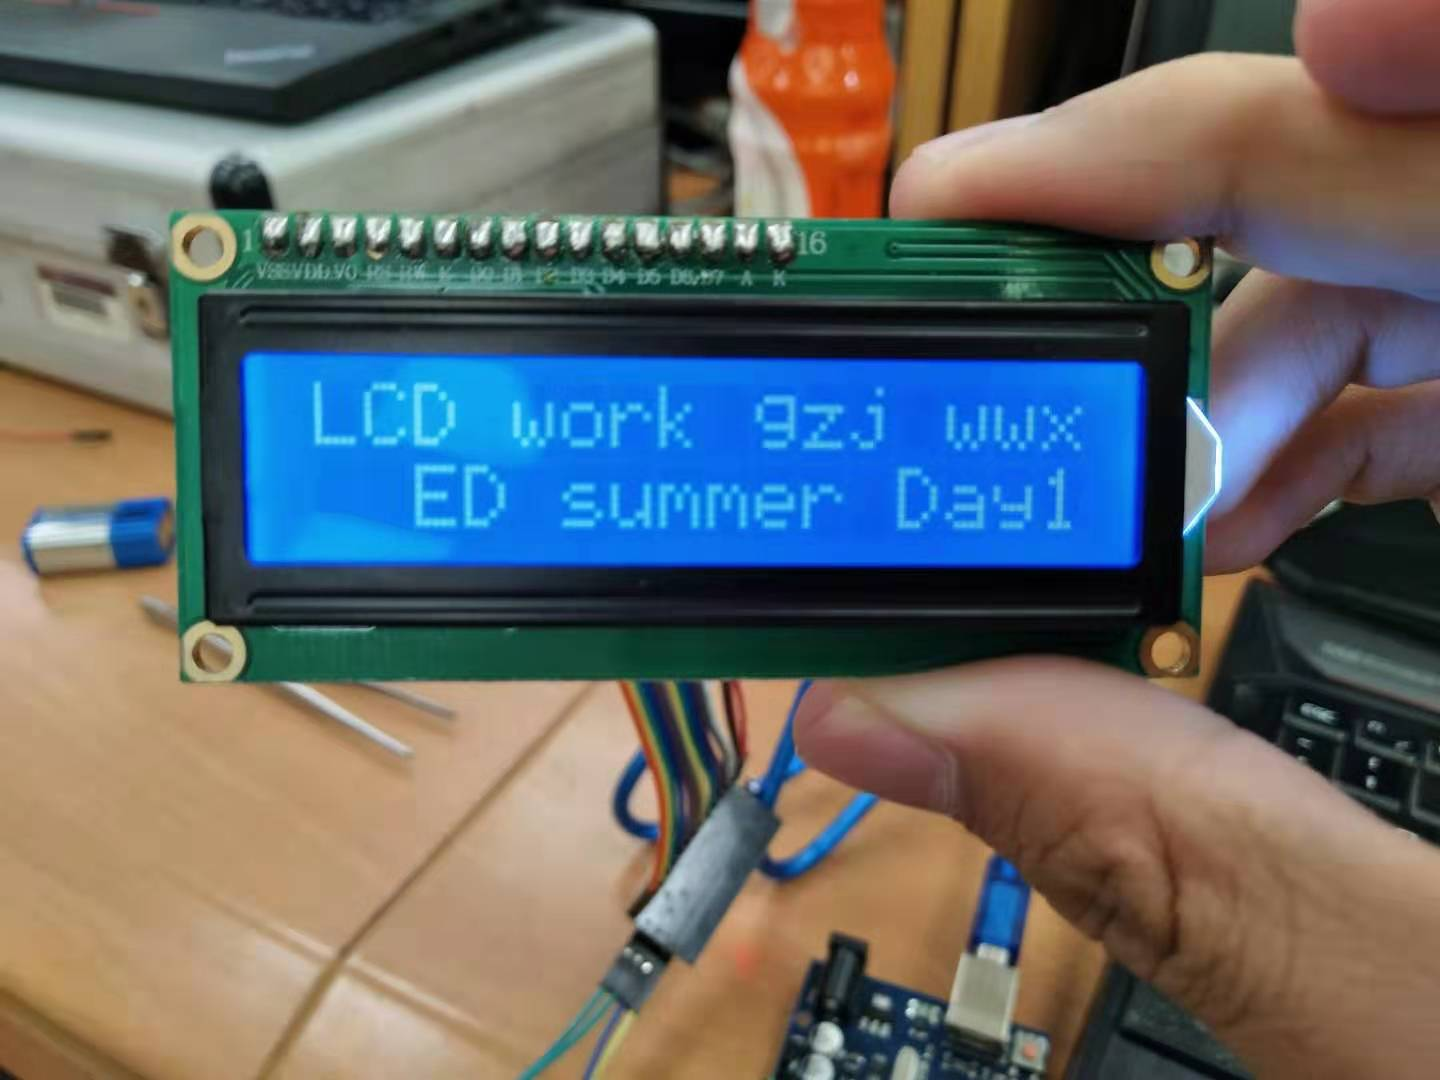
\includegraphics[width = 0.53\textwidth]{chuan2.jpg}
  \caption{LCD字符显示}
\end{figure}
起初并不能显示,后来我们很快发现是转接板电位器的问题,转接板电位器直接控制了LCD显示的亮度,因此在使用镊子改变电位到合适的亮度后便能观察到字符。在能够显示字符后,我们进一步结合上午的学习进行了串口LCD通信联调,使得在键盘上实时输入字符在LCD上进行显示,这是我们之后显示模块的重要基础,我们拍摄成果的照片如下:
\begin{figure}[H]
  \centering
  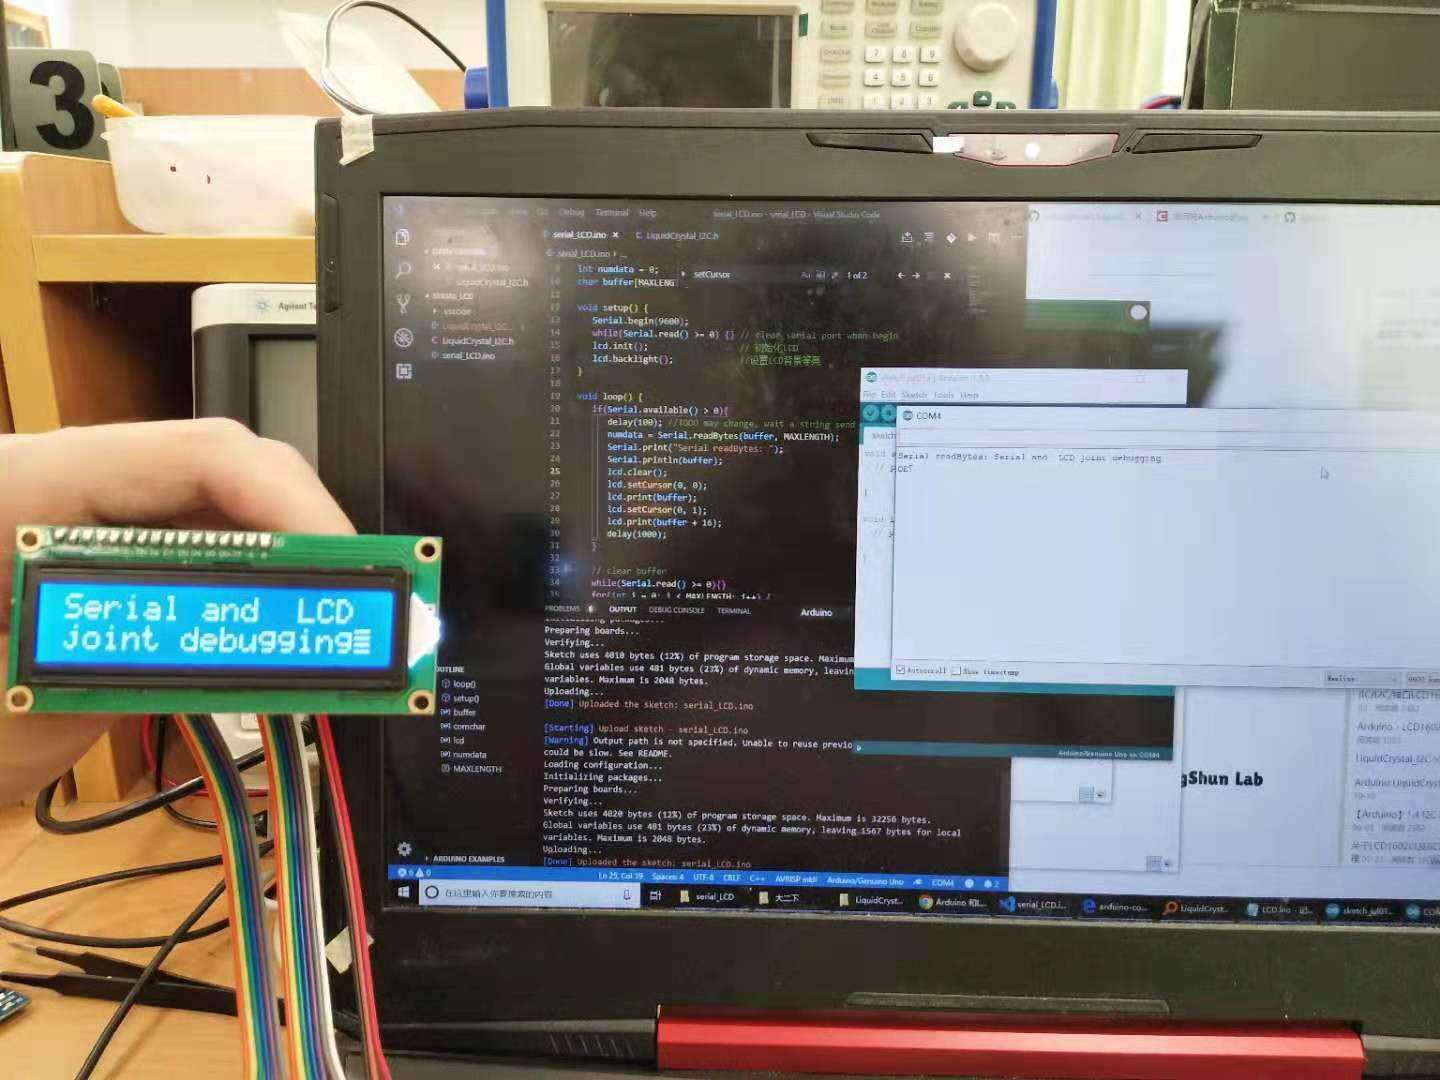
\includegraphics[width = 0.53\textwidth]{chuan1.jpg}
  \caption{LCD串口通信联调}
\end{figure}
另一方面,我们组在调试LCD的同时,对电源管理电路进行了实际的检测,我们计划使用9V的干电池,而恰好在实验室中找到一块电源管理的模块,能够在小于12V输入的情况下,输出5V/3.3V的直流电压,我们类比于电网$10\%$的波动,使用$8V\sim 10V$的50Hz正弦波作为输出,观察两输出的电压情况,结果十分令人满意,根据示波器的显示,以及自动测量的结果,能够得到纹波非常小的直流电压,并十分接近其标称的输出,记录如下图所示:
\begin{figure}[H]
  \begin{minipage}[t]{0.45\linewidth}
      \centering
      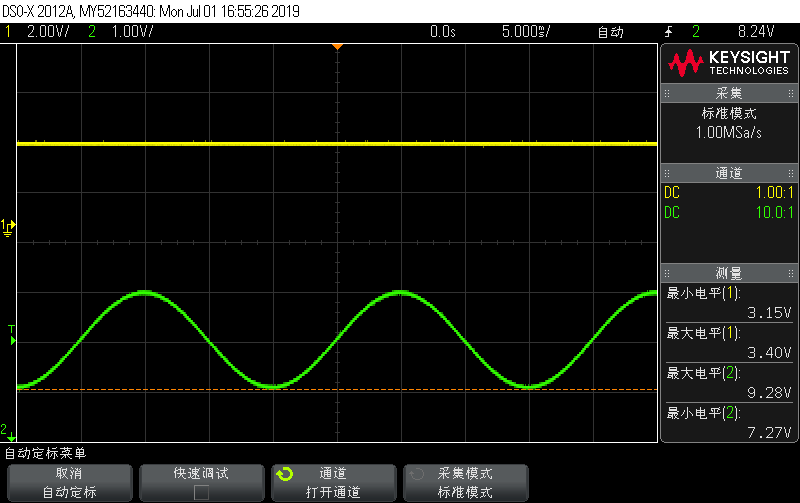
\includegraphics[width=6cm]{dy1.png}
      \caption{3.3V稳压输出}
  \end{minipage}%
      \hfill
  \begin{minipage}[t]{0.45\linewidth}
      \centering
      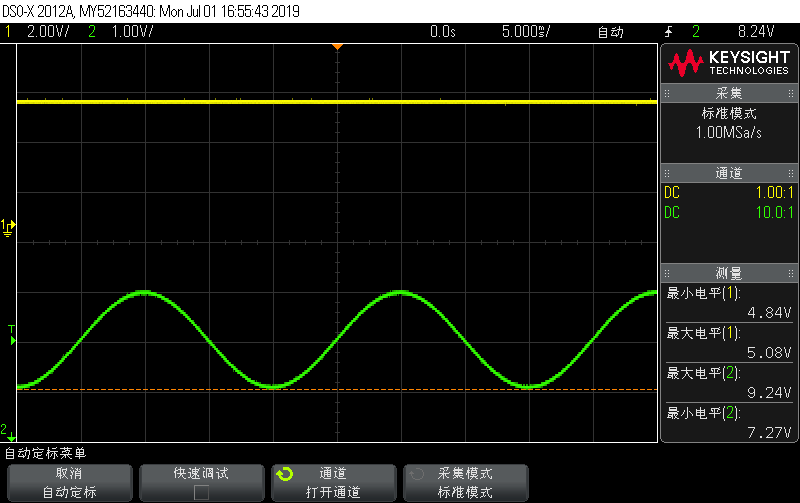
\includegraphics[width=6cm]{dy2.png}
      \caption{5V稳压输出}
  \end{minipage}
\end{figure}
其中黄色线为稳压输出,绿色线为输入,验证了该电源管理模块能够提供理想的供电电压,在TI公司的样片到来之前为我们的电源管理提供了替代。

在下午收工以后我们另外找到一片蓝牙模块,计划于明天开启蓝牙模块的调试以及DHT11的湿度模块的调试,并通过LiquidCrystal库编写代码,实现自己需要的函数的头文件。

\end{diary}

\begin{diary}{2019.07.02上午}{DHT11温湿模块与蓝牙模块调试}
\par{}电子设计小学期工作日的第二个上午,我们明显加快了调试的进度,在昨天初步调试LCD1602后,今天我们进一步同时开始调试蓝牙模块和DHT11温湿模块。

首先,上午蓝牙模块的调试并不是十分顺利,中间遇到了一些连接的问题,进度稍慢,而温度湿度传感器模块借助于Arduino官网可查找的dht11的库,可以很快的进行实现。我们设置没两秒更新并发送一次数据,可以在串口接受到数据。之后便很方便地将数据

为了验证其正确性,我们将传感器分别在室内与室外进行了测量,结果表明室外比室内温度大约高$3^\circ C$左右,湿度也稍高于室内,符合实际情况,测量结果如下图\ref{img1}记录:
\begin{figure}[H]
  \centering
  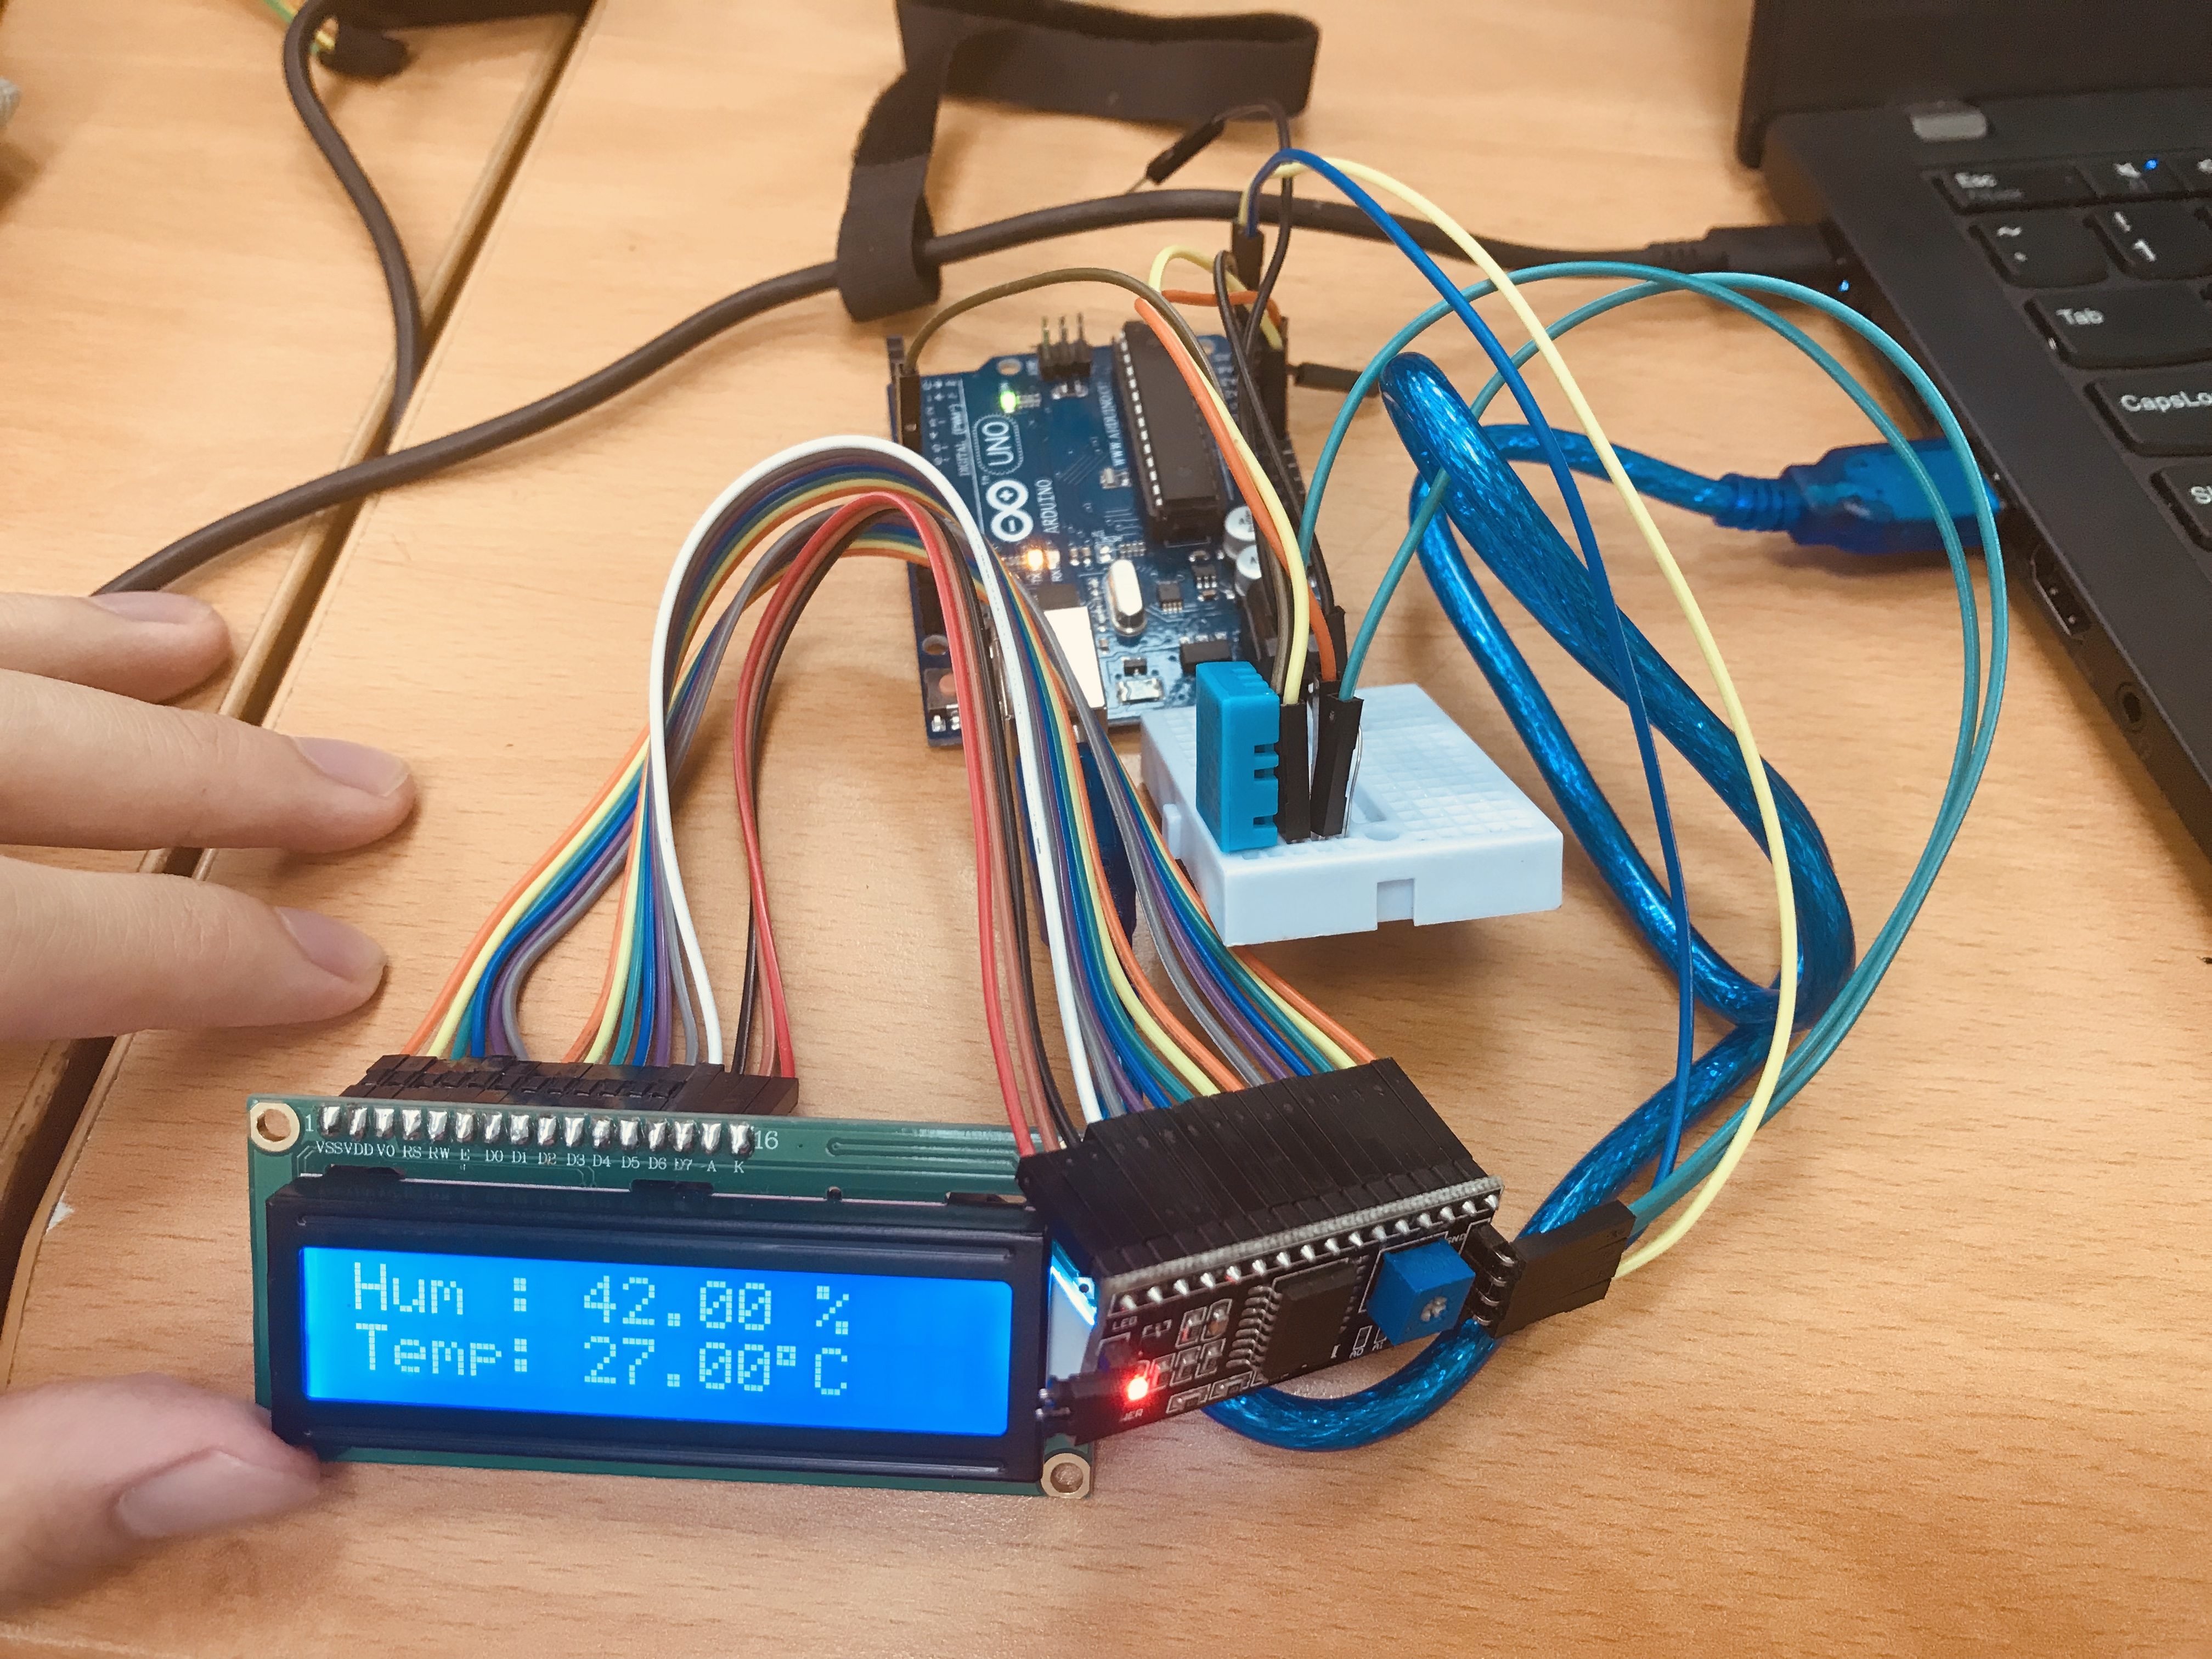
\includegraphics[width = 0.53\textwidth]{temp1.jpg}
  \caption{温度湿度测量与LCD显示}
  \label{img1}
\end{figure}

该LCD显示了当前教室的室温和室内湿度。
整体上温度湿度模块由于能够直接输出校准后的数字信号,所以调试过程比较顺利,只是在单位的输出时$^{\circ}C$的符号难以直接输出,库中的print()函数无法输出该字符,需要去自定义字符,否则会输出响应的日文,因此我最终采用了print((char)233)在其中一格的$5\times 7$矩阵先输出“度”的上标,再输出C来完成单位的显示。

此外,我们修改了$LiquidCrystal\_I2C$库的内容,将其精简并增加了和串口联调的功能,成为我们可以使用的$serial\_lcd$库,其中的函数实现原理大致与官方库相同。此后该模块恰好能够利用该屏幕进行显示,因此我们考虑了一下多模块测量的显示方法,我们选用TTP226电容触摸开关进行显示内容的选择,不同的开关控制不同内容的显示,因此我们目前手头只有TTP224,并用其进行测试其触摸效果,结果十分令人满意。

而另一模块,蓝牙模块的调试,能够初步和设备进行连接,但基于Arduino进行数据通讯仍具有一定的问题,有待下午进一步调试。

\end{diary}


\begin{diary}{2019.07.02下午}{蓝牙模块调试和系统架构细节讨论}

在下午我们完成了蓝牙模块的调试,经过排查,发现是使用的蓝牙模块已经进行了配置,和出厂设置不同,厂方给出的设置方案不能直接使用。在简单了解AT指令集后,我们迂回使用USB转TTL的芯片,先对蓝牙模块进行恢复出厂设置,便可按照厂方文档进行调试。按照应用情景,我们将蓝牙模块设置为从机,波特率设置为9600(之后可能会调节到更低以节省功耗),简单测试了手机通过蓝牙模块、电脑通过蓝牙模块与arduino的通信,顺利完成数据的收发并能做出简单的响应,可以预料到能与后续的模块完成连接。

此外,气压传感器BMP180的特性测试和简单实用调试也在今天下午完成。此外在考虑微波雷达探测人体存在的实际情况,我们认为可能需要做一定的角度的扫描检测,故而在实验末尾简单阅读了舵机的工作原理和操作例程,这是一个控制模块,可以预料到调试环节不一定顺利。但是这是一个数字驱动的模块,可以在今晚先将大部分功能点实现,其他的预想功能如根据雷达信号的反旋转舵机,需要之后联调实现。

最后,已经看到的情况是,由于外设较多,arduino的IO资源已经有些紧张,而且各外设的使用方式不一,有直接用IO功能进行读写,有用I2C进行通信。我们敲定方案是用IO转I2C和I2C扩展板,实现一个统一的数据总线结构,方便整体系统调试。另外我们还需要一个数据存储媒介给仪器记录实验数据。所以在今天下午实验结束后,我们还去中关村中发市场进行了相关器件的采购。

\end{diary}


\begin{diary}{2019.07.03上午}{舵机、SD卡、LCD12864、红外收发调试}
  
电子设计小学期工作日的第三个上午,我们继续对已有的模块进行测试。我们在昨天的采购时重新购置了一块较大的液晶显示屏,型号为LCD12864,是一块分辨率为128*64的显示屏,并带有中文字库,相比与1602具有更大的优势,首先我们先去将其20引脚焊好排针,之后我们利用了已有的一个简单库函数,并且对其进行函数的补充与丰富,例如清除光标等函数,并对其进行了显示的测试,测试结果能够清楚的显示如下图\ref{img2},但是发现该屏幕对电磁干扰非常敏感,在硬件接线有扰动或者其他电磁干扰的情况下,会出现乱码的情况,这是我们进一步需要解决的问题。
\begin{figure}[H]
  \centering
  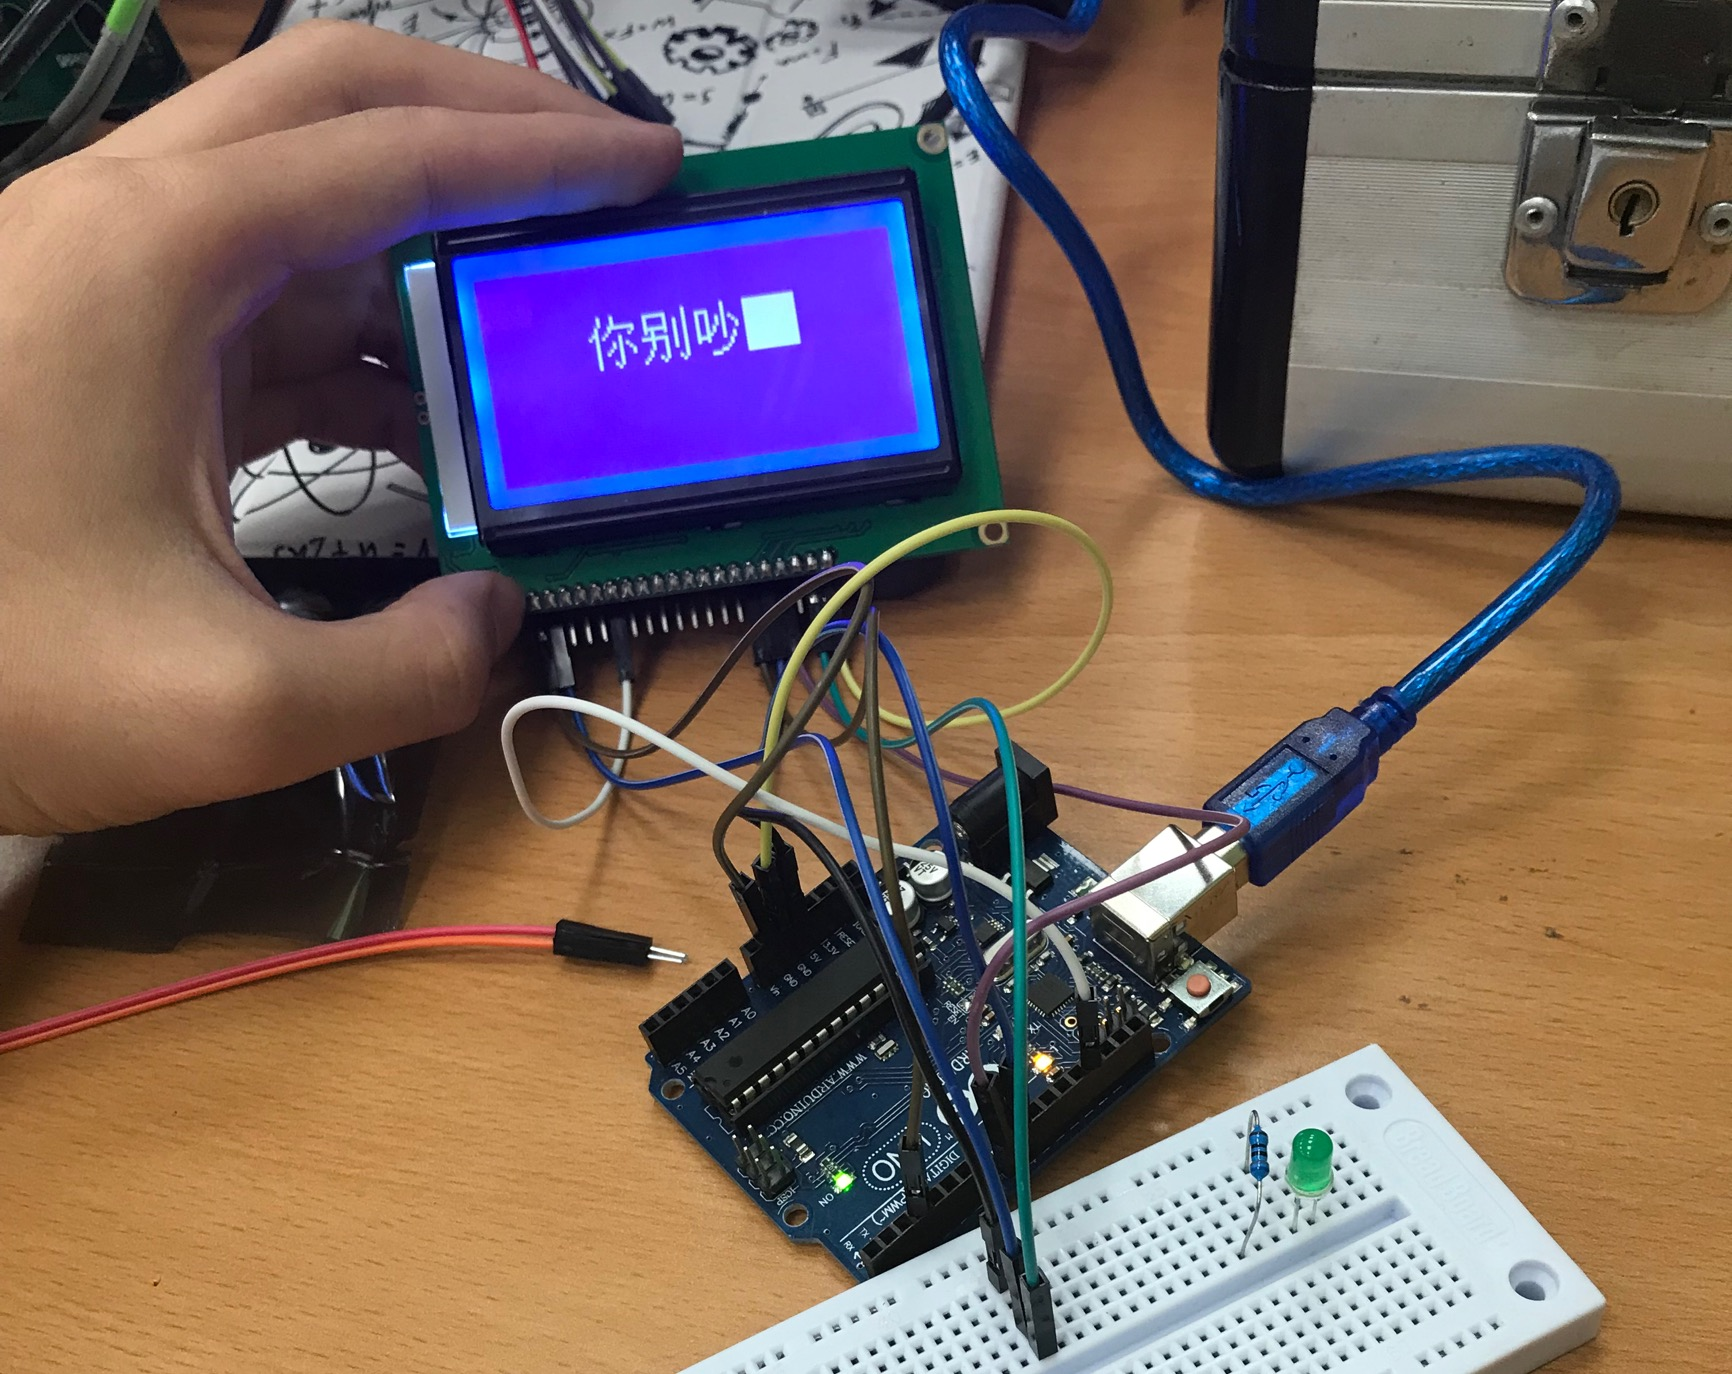
\includegraphics[width = 0.53\textwidth]{12864.jpg}
  \caption{12864显示}
  \label{img2}
\end{figure}

除此之外,我们调试使得舵机能够正常运转,我们希望借助180$^{\circ}$旋转的舵机能够帮助微波雷达模块对室内的人体进行感应与检测,扩大其检测范围。在调通舵机后,我们开始了对SD卡存储的调试,初步能够实现通过Arduino将数据发送的SD卡进行存储。并且在舵机模块和SD卡模块的类库的使用中,我们注意到从类库生成的对象较大(一个舵机大约占用动态内存的20\%、一个SD文件对象大约占用动态内存的50\%),故而我们讨论了两种解决方案,第一是精简类库,减少内存消耗,二是使用PROGMEM后缀,将变量存储在flashrom中。第二个解决方案用于对读写实时性的要求不高的场景,初步确认SD卡文件对象内存占用大的问题可以使用这个方式得以解决。这是因为将测量数据转存到SD卡的操作本身就是外存文件操作,速度较低。而舵机对象的问题推迟到最后联调时视情况解决。此外我们还进行了红外收发模块的调试和标定:得到编码如下:

\begin{figure}[H]
  \centering
  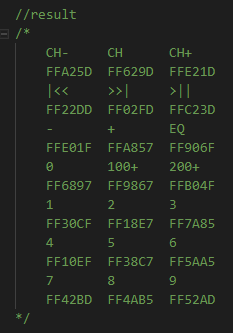
\includegraphics[width = 0.2\textwidth]{controller_code.png}
  \caption{红外遥控编码}
\end{figure}

并且我们进一步讨论总线的管理方法,由于IO资源较少,而待测量变化频率一般较低,我们希望能够在每次轮询周期内利用一根总线分别选通各传感器进行数据传输,因此我们需要搭建数据选择电路,为此我们在午饭时再次前往中发市场购置数据选择器等器件。

\end{diary}

\begin{diary}{2019.07.03下午}{元件增购与总线结构讨论}
  
  根据课上所学的知识,我们在中发市场增购了八输入数据选择器74151,用做输入总线的设计。此外采购了GPIO转I2C的芯片PCF8574。I2C在LCD1602调试时我们接触到的一个串行通信协议。在下午的正是调试中,我们两路并行进行,一方面对购得的元件进行逻辑测试,另一方面学习理解I2C协议。以下是在PCF8574的数据手册中截图得到的关于I2C的介绍。大约分为主机发送起止命令、选择地址和读写模式,以及从机被读或被写时按8位数据位一位应答位的串行数据传输形式。

\begin{figure}[H]
  \centering
  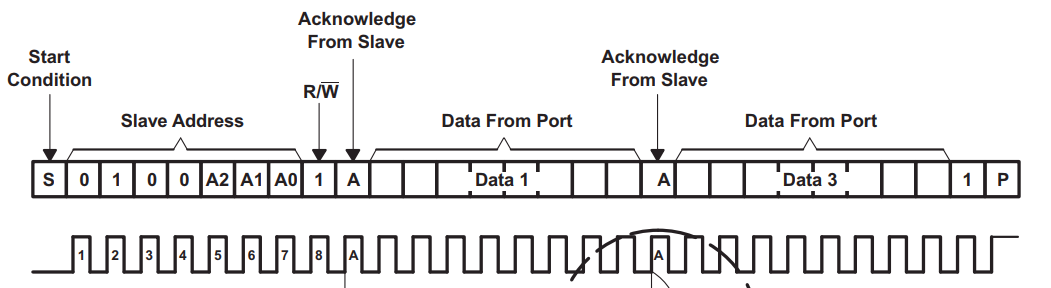
\includegraphics[width = 0.8\textwidth]{I2C.png}
  \caption{I2C数据传输举例(从数据手册中摘录)}
\end{figure}

在简单讨论后,我们决定先试用I2C进行总线管理。主要出于以下几个目的:

\begin{enumerate}
  \item I2C适用于通信速率低的情景,在轮询传感器时,符合这个特点。
  \item I2C是相对主流的通信协议,可以方便后续拓展。
  \item I2C协议读写均支持,是更完整意义上的总线形式,比起我们用数据选择器设计的只读总线结构更为合理,也可以把读传感器值和内容显示等读写操作统一在一个时序中,让程序更为统一。
  \item I2C协议要求我们对时序电路有更好的理解,我们也想在这方面挑战一下自己。
\end{enumerate}

\end{diary}


\begin{diary}{2019.07.04上午}{I2C总线协议理解与讨论}

在网购元件到来前的最后一个上午,我们首先进一步研究I2C总线协议,为我们之后的总线架构做出准备与铺垫。我们阅读并参透了LiquidCrystal的库函数,进一步参透了解I2C传输协议。

除此之外,我们另一路开始为下午的模块调试进行准备,计划在下午能够完成所有模块的调试使得明天可以进行各模块的联调。首先查阅了GP2Y1050AU0F的模拟输出特性,以此为基础先编写好程序,并进一步连接其接线,由于我们已知其为模拟输出,自然考虑到传感器的输出会受到噪声的影响,为了改进输出特性,我们提前设计好了VCVS低通滤波电路,滤波特性如下:
\begin{figure}[H]
  \centering
  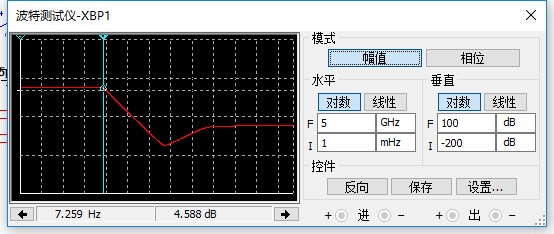
\includegraphics[width = 0.75\textwidth]{bote.png}
  \caption{低通滤波特性}
\end{figure}

可见我们已经能够实现低通滤波的仿真,使得该模块的模拟输出稳定,并且在之后综合比较了LCD1602和LCD12864的显示效果以及调试难度,由于12864的显示常常因电磁干扰而显示乱码,我们仍决定采用1602。在上午的工作接近末尾时,我们大概完整的阅读并理解完I2C协议与LCD显示的库函数,我们在网上购置的模块也终于到来,为我们开发工作的进度有进一步推动。

\end{diary}

\begin{diary}{2019.07.04下午}{PM2.5传感器、微波雷达、光强测量电路的调试}
  
下午模块一到,我们便首先对PM2.5检测的GP2Y1050AU0F传感器的特性进行标定。室内空气质量好,故传感器的模拟输出较低,且用示波器看不到明显变化。在回忆了传感器的原理,是通过对管对自己发射的光信号进行放大,而收集槽中的灰尘会部分挡光导致输出示数变化。故而我们简单用铅笔伸入收集槽的方法对传感器特性进行测试。下图为伸入铅笔后的,滤波前和滤波后的输出:

\begin{figure}[H]
  \begin{minipage}[H]{0.48\textwidth}
    \begin{figure}[H]
      \centering
      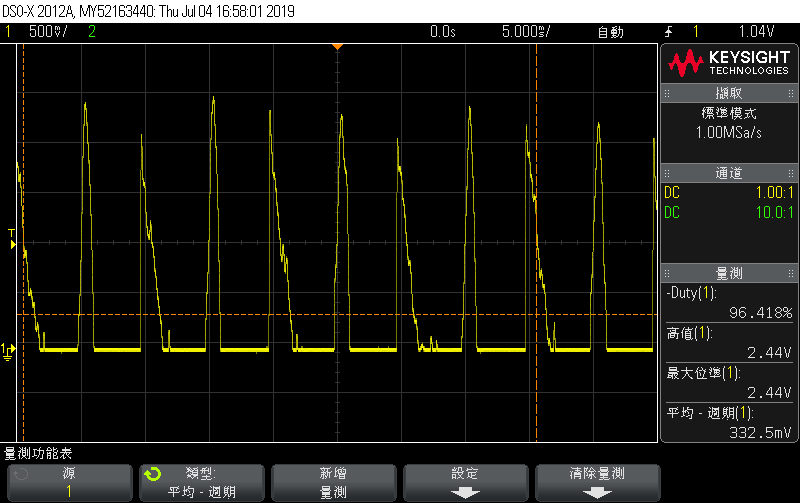
\includegraphics[width = 0.8\textwidth]{before_fliter.png}
      \caption{灰尘传感器滤波前输出}
    \end{figure}
  \end{minipage}
  \begin{minipage}[H]{0.48\textwidth}
    \begin{figure}[H]
      \centering
      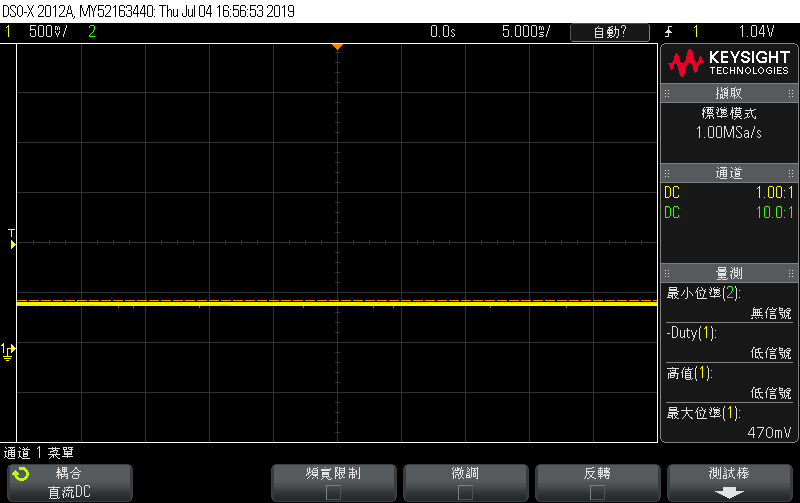
\includegraphics[width = 0.8\textwidth]{after_fliter.png}
      \caption{灰尘传感器滤波后输出}
    \end{figure}
  \end{minipage}
\end{figure}

可以看到,滤波后输出质量明显提高。并且可以想到的是,在本次实验中的噪声主要来自铅笔的晃动,而实际测量中的噪声可能来自空气颗粒的随机运动,应该会是更大的噪声,故而进行这次滤波是很有必要的。

微波雷达的生物探测功能已经进行了验证,在所需范围内有生物移动时会得到高电平输出,并且其穿透探测的功能也得到了验证。但是由于小组中一人的工作台的示波器工作异常,故没有记录详细波形。

最后是光强测量电路的设计、仿真和调试。手边拥有的光敏元件是光敏电阻,在查阅了光敏电阻的光敏特性曲线,其理想的关系应当是

\begin{equation*}
  \ln(\frac{R}{R_0}) \propto \ln(\frac{I}{I_0})
\end{equation*}

最直接的想法是用分压关系将反映成电阻变化的光强变化作为电压信号,接入后级的放大和滤波电路后得到检测信号。但分压网络的缺点是会在分子和分母都出现变化的电阻,故而电压信号和待测物理量不是线性关系,需要后级的数字系统用计算处理。而在本例中,问题更为复杂了,因为待测物理量和电阻值的变化并非线性关系,导致了一个超越方程,难以求解。若使用计算机上常用的方式,即基于试根的方法会比较占用MCU本就不多的计算资源,很得不偿失。故而转换思路,使用555压控振荡器做电阻-频率转换。首先进行仿真验证,搭接如下电路。

\begin{figure}[H]
  \centering
  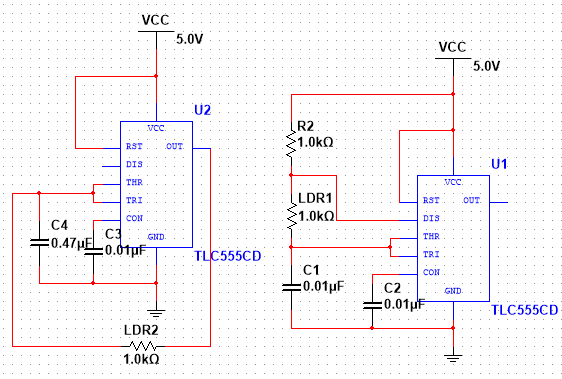
\includegraphics[width = 0.618\textwidth]{555_sim.jpg}
  \caption{基于555多谐振荡电路的光强检测计}
\end{figure}

图中标注LDR的即为光敏电阻,左侧方案更为简洁,并且得到的是占空比$50\%$的方波,更好进行检测。进行优先的仿真和调试。简单的数学推导后得到输出波形振荡周期$T$与光敏电阻值$R$成正比,是一个简单的关系。故而可以避免解超越方程的尴尬。仿真振荡波形如下,但由于实际电路需要对光强进行标定,实际测量的调试在明天携带进行,仿真波形仅用于确认电路可正常工作。此外,基于555的测量电路还有在光敏电阻上电压值较为恒定,输出电平标准稳定不容易损害后级电路和低功耗的特点,是我们认为较之于基于分压电路的设计方案更好更简洁的解决方案。

\begin{figure}[H]
  \centering
  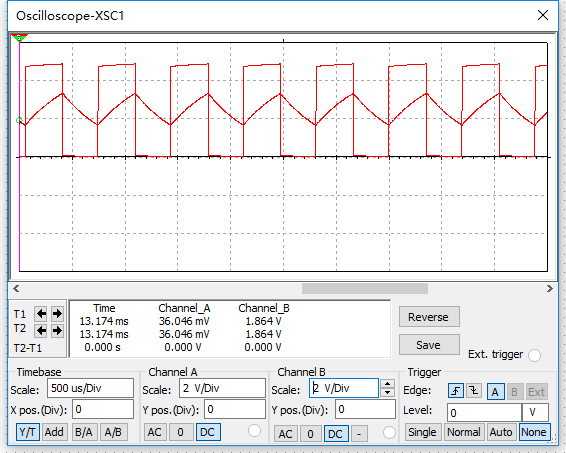
\includegraphics[width = 0.618\textwidth]{555_sim_osc.jpg}
  \caption{555多谐振荡光强测量电阻仿真波形图}
\end{figure}

\end{diary}
\begin{diary}{2019.07.05上午}{模块联调初步搭建与电源管理模块PCB设计}

  \par{}在工作日的第五个上午我们在调试通过各种模块串口数据收发的基础上,开始了所有模块的联合调试,此外,我们在昨晚收到了TI公司的样片,电源管理模块使用的芯片TPSM84,也进一步对电源管理模块进行测试。

  首先在面包板上搭建电源管理模块的电路,输入$8\sim 10$V的正弦波,观察稳定输出的结果,如下图所示:

\begin{figure}[H]
  \centering
  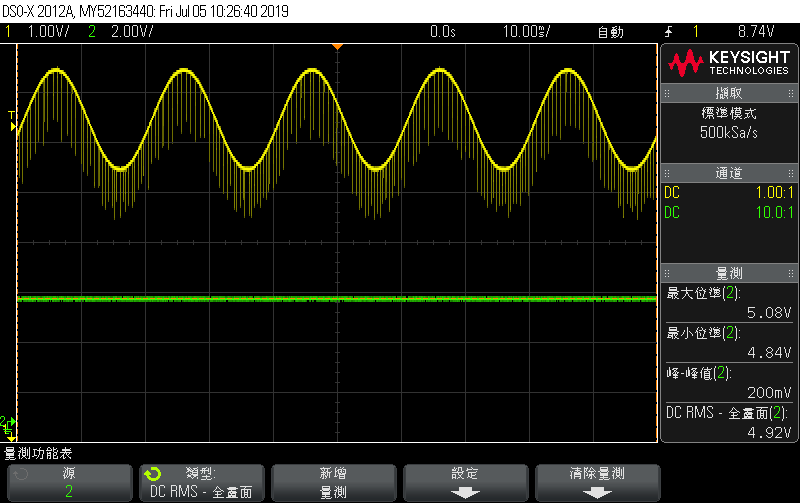
\includegraphics[width = 0.618\textwidth]{dianyuan.png}
  \caption{电源管理模块}
\end{figure}

在输入正弦波存在毛刺的情况下,输出电压非常稳定,波动在毫伏级别,因此我们也验证了该模块能够正常工作,因此,我们计划将电源管理模块单独设计出一块PCB板进行系统的供电,由于本身的电源管理模块部分比较简单,因此也便于我们去添加额外的开关和电源指示灯,我们在上午绘制好了电源管理模块的PCB图并送去制版,如下图所示:
\begin{figure}[H]
  \centering
  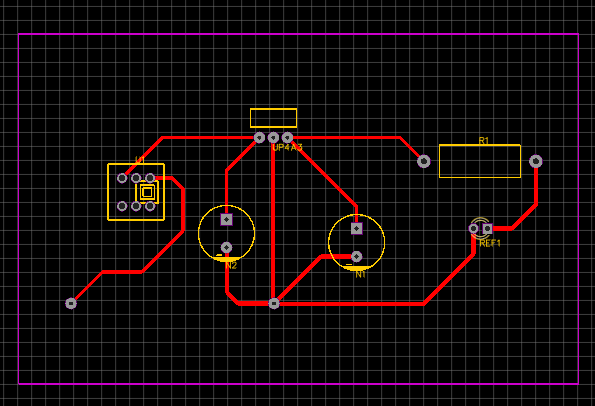
\includegraphics[width = 0.58\textwidth]{pcb.png}
  \caption{电源管理模块PCB绘制}
\end{figure}
在PCB绘制的过程中,由于我们无法从元件库找到TPSM84芯片,因此查阅其datasheet换算单位后自己制作出了TPSM84的PCB模块,并且后来由于添加开关我们现找了自锁的按动开关,查阅其引脚和内部连接后进行接线,初次绘制PCB耗费了一定的时间。

另一路工作首先对基于555的光强检测电路进行了简单的实物搭接和收尾验证,得到波形如下:

\begin{figure}[H]
  \begin{minipage}[H]{0.48\textwidth}
    \begin{figure}[H]
      \centering
      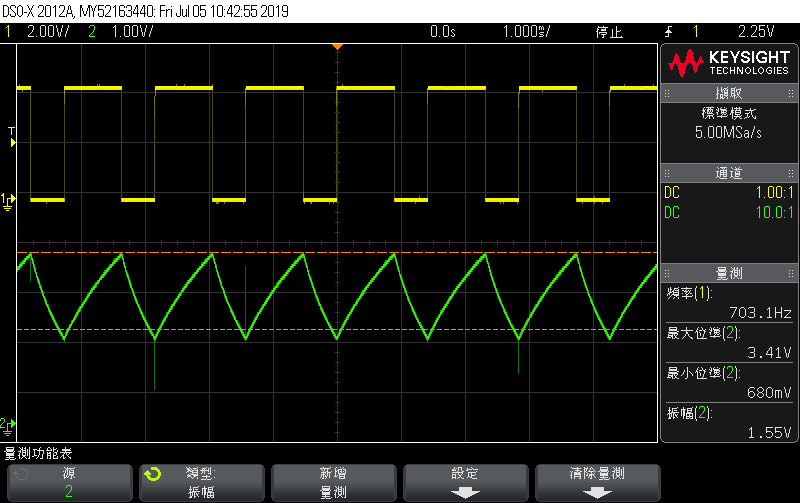
\includegraphics[width = 0.8\textwidth]{light_osc.png}
      \caption{光强检测电路波形(室内正常环境)}
    \end{figure}
  \end{minipage}
  \begin{minipage}[H]{0.48\textwidth}
    \begin{figure}[H]
      \centering
      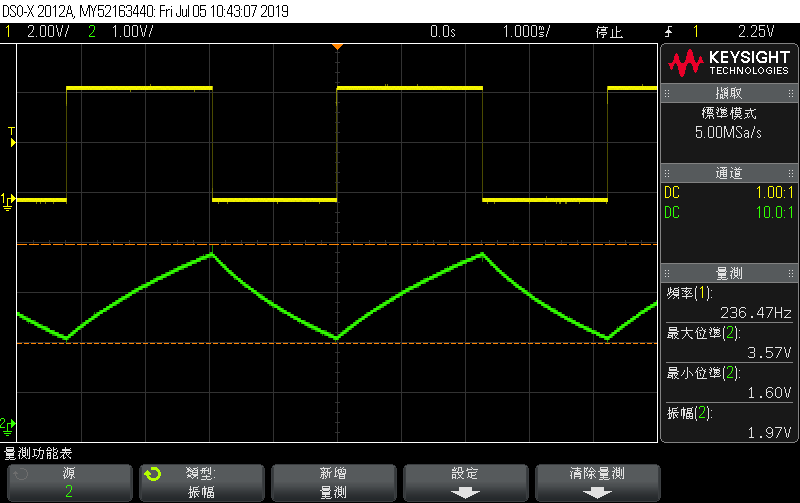
\includegraphics[width = 0.8\textwidth]{dark_osc.png}
      \caption{光强检测电路波形(遮挡光敏电阻)}
    \end{figure}
  \end{minipage}
\end{figure}

可以从波形可以定性看到,由于光强减弱,光敏电阻阻值的增加,振荡周期增加,频率减小,符合定性规律。另外一方面,参考室内$300\text{lx}$,而遮挡时,近似看为野外室外环境光强$1lx$扣除偏移量,验证其对数值的近似线性关系。

之后的工作计划于面包板上先实现硬件的连接,随着硬件的搭建我们同时开始软件方面的引脚分配,初步在无总线的情况下在Arduino串口轮询读取数据,若其能够联合正常工作并读取数据,则可进一步设计PCB和添加总线方案。我们已经在面包板上完成了基于555的光强检测计,DHT温度湿度模块,BMP180气压检测和PM2.5模块的低通滤波部分,以及红外遥控模块,如下图所示:
\begin{figure}[H]
  \centering
  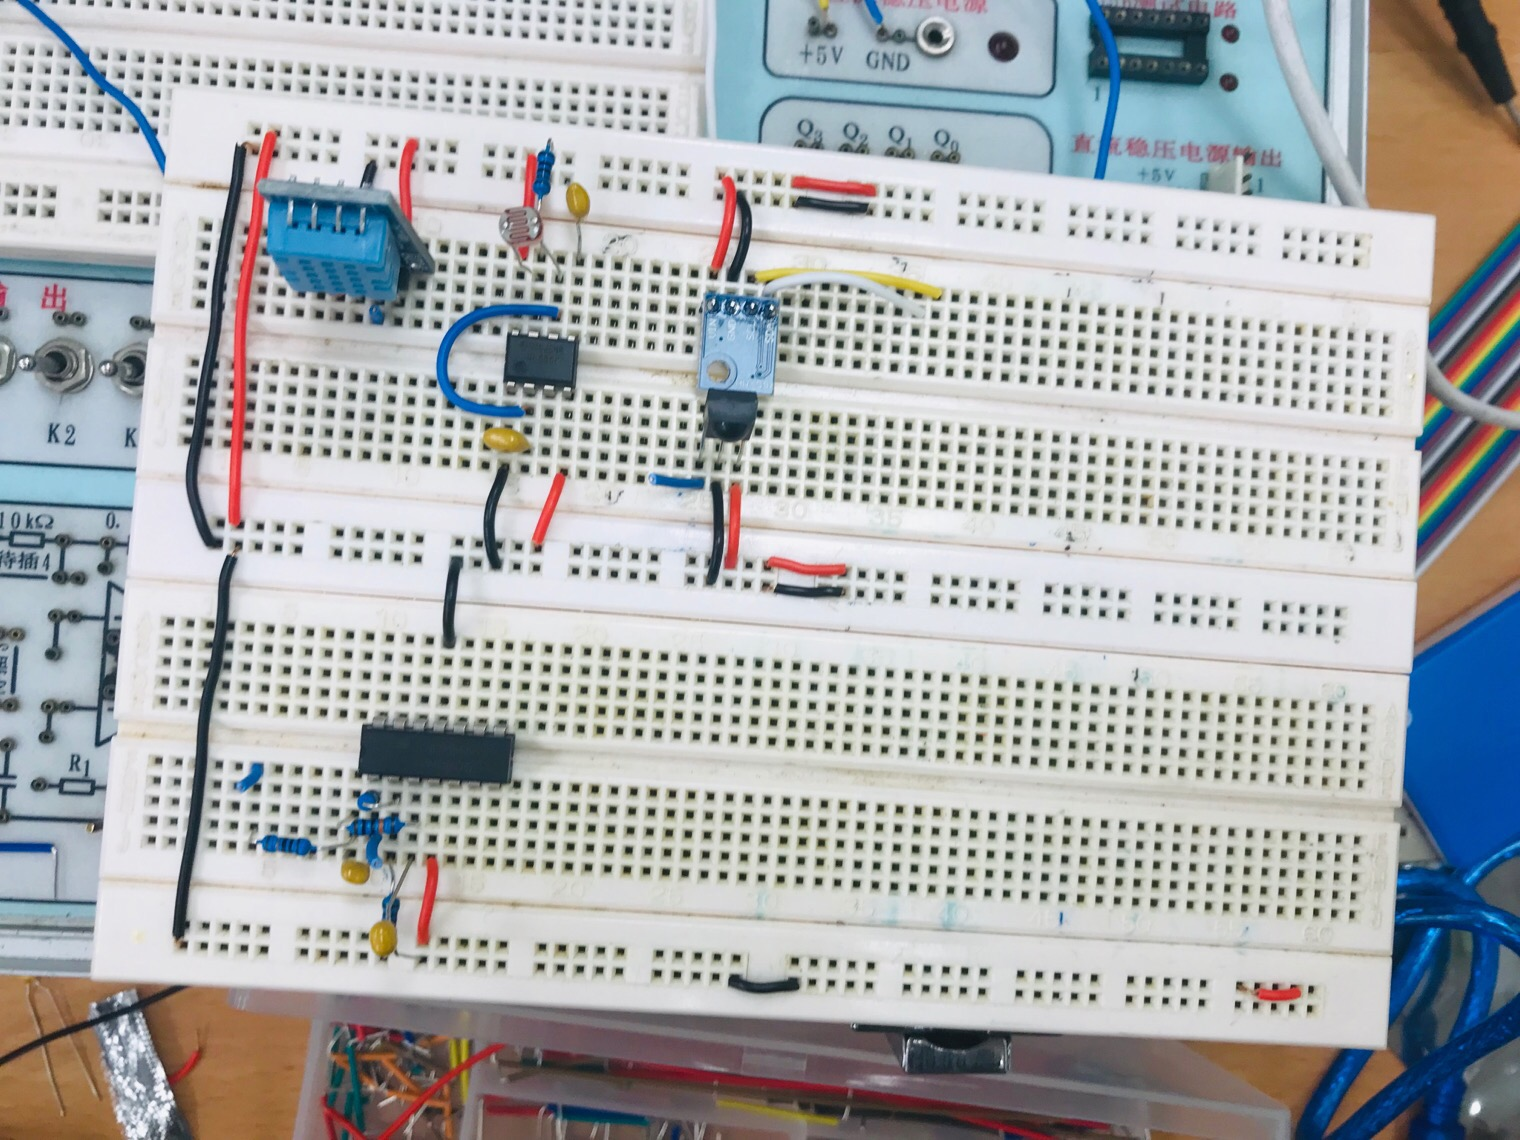
\includegraphics[width = 0.58\textwidth]{lianhe.jpg}
  \caption{联合调试部分硬件}
\end{figure}
在下午的工作中我们将进一步进行搭建以及编写ino进行串口数据读取,如果PCB制作完成则会进一步焊接与测试。


\end{diary}

\begin{diary}{2019.07.05下午}{模块联调}

下午实验开始后,我们打印的PCB很快就做好了,所以我们兵分两路,一路进行PCB的焊接,一路继续进行联调电路的搭接。最后的搭接完成后,我们在面包板上放置了基于555的光强检测计,DHT温度湿度模块,BMP180气压检测和PM2.5模块和其配套的低通滤波器,红外接收管、微波雷达和按键和其对应总线管理的数字模块。如下图(图片为实验结束后拍摄,当时为了携带方便,体积较大的PM2.5传感器和疑似烧坏的按键没有连接)

\begin{figure}[H]
  \centering
  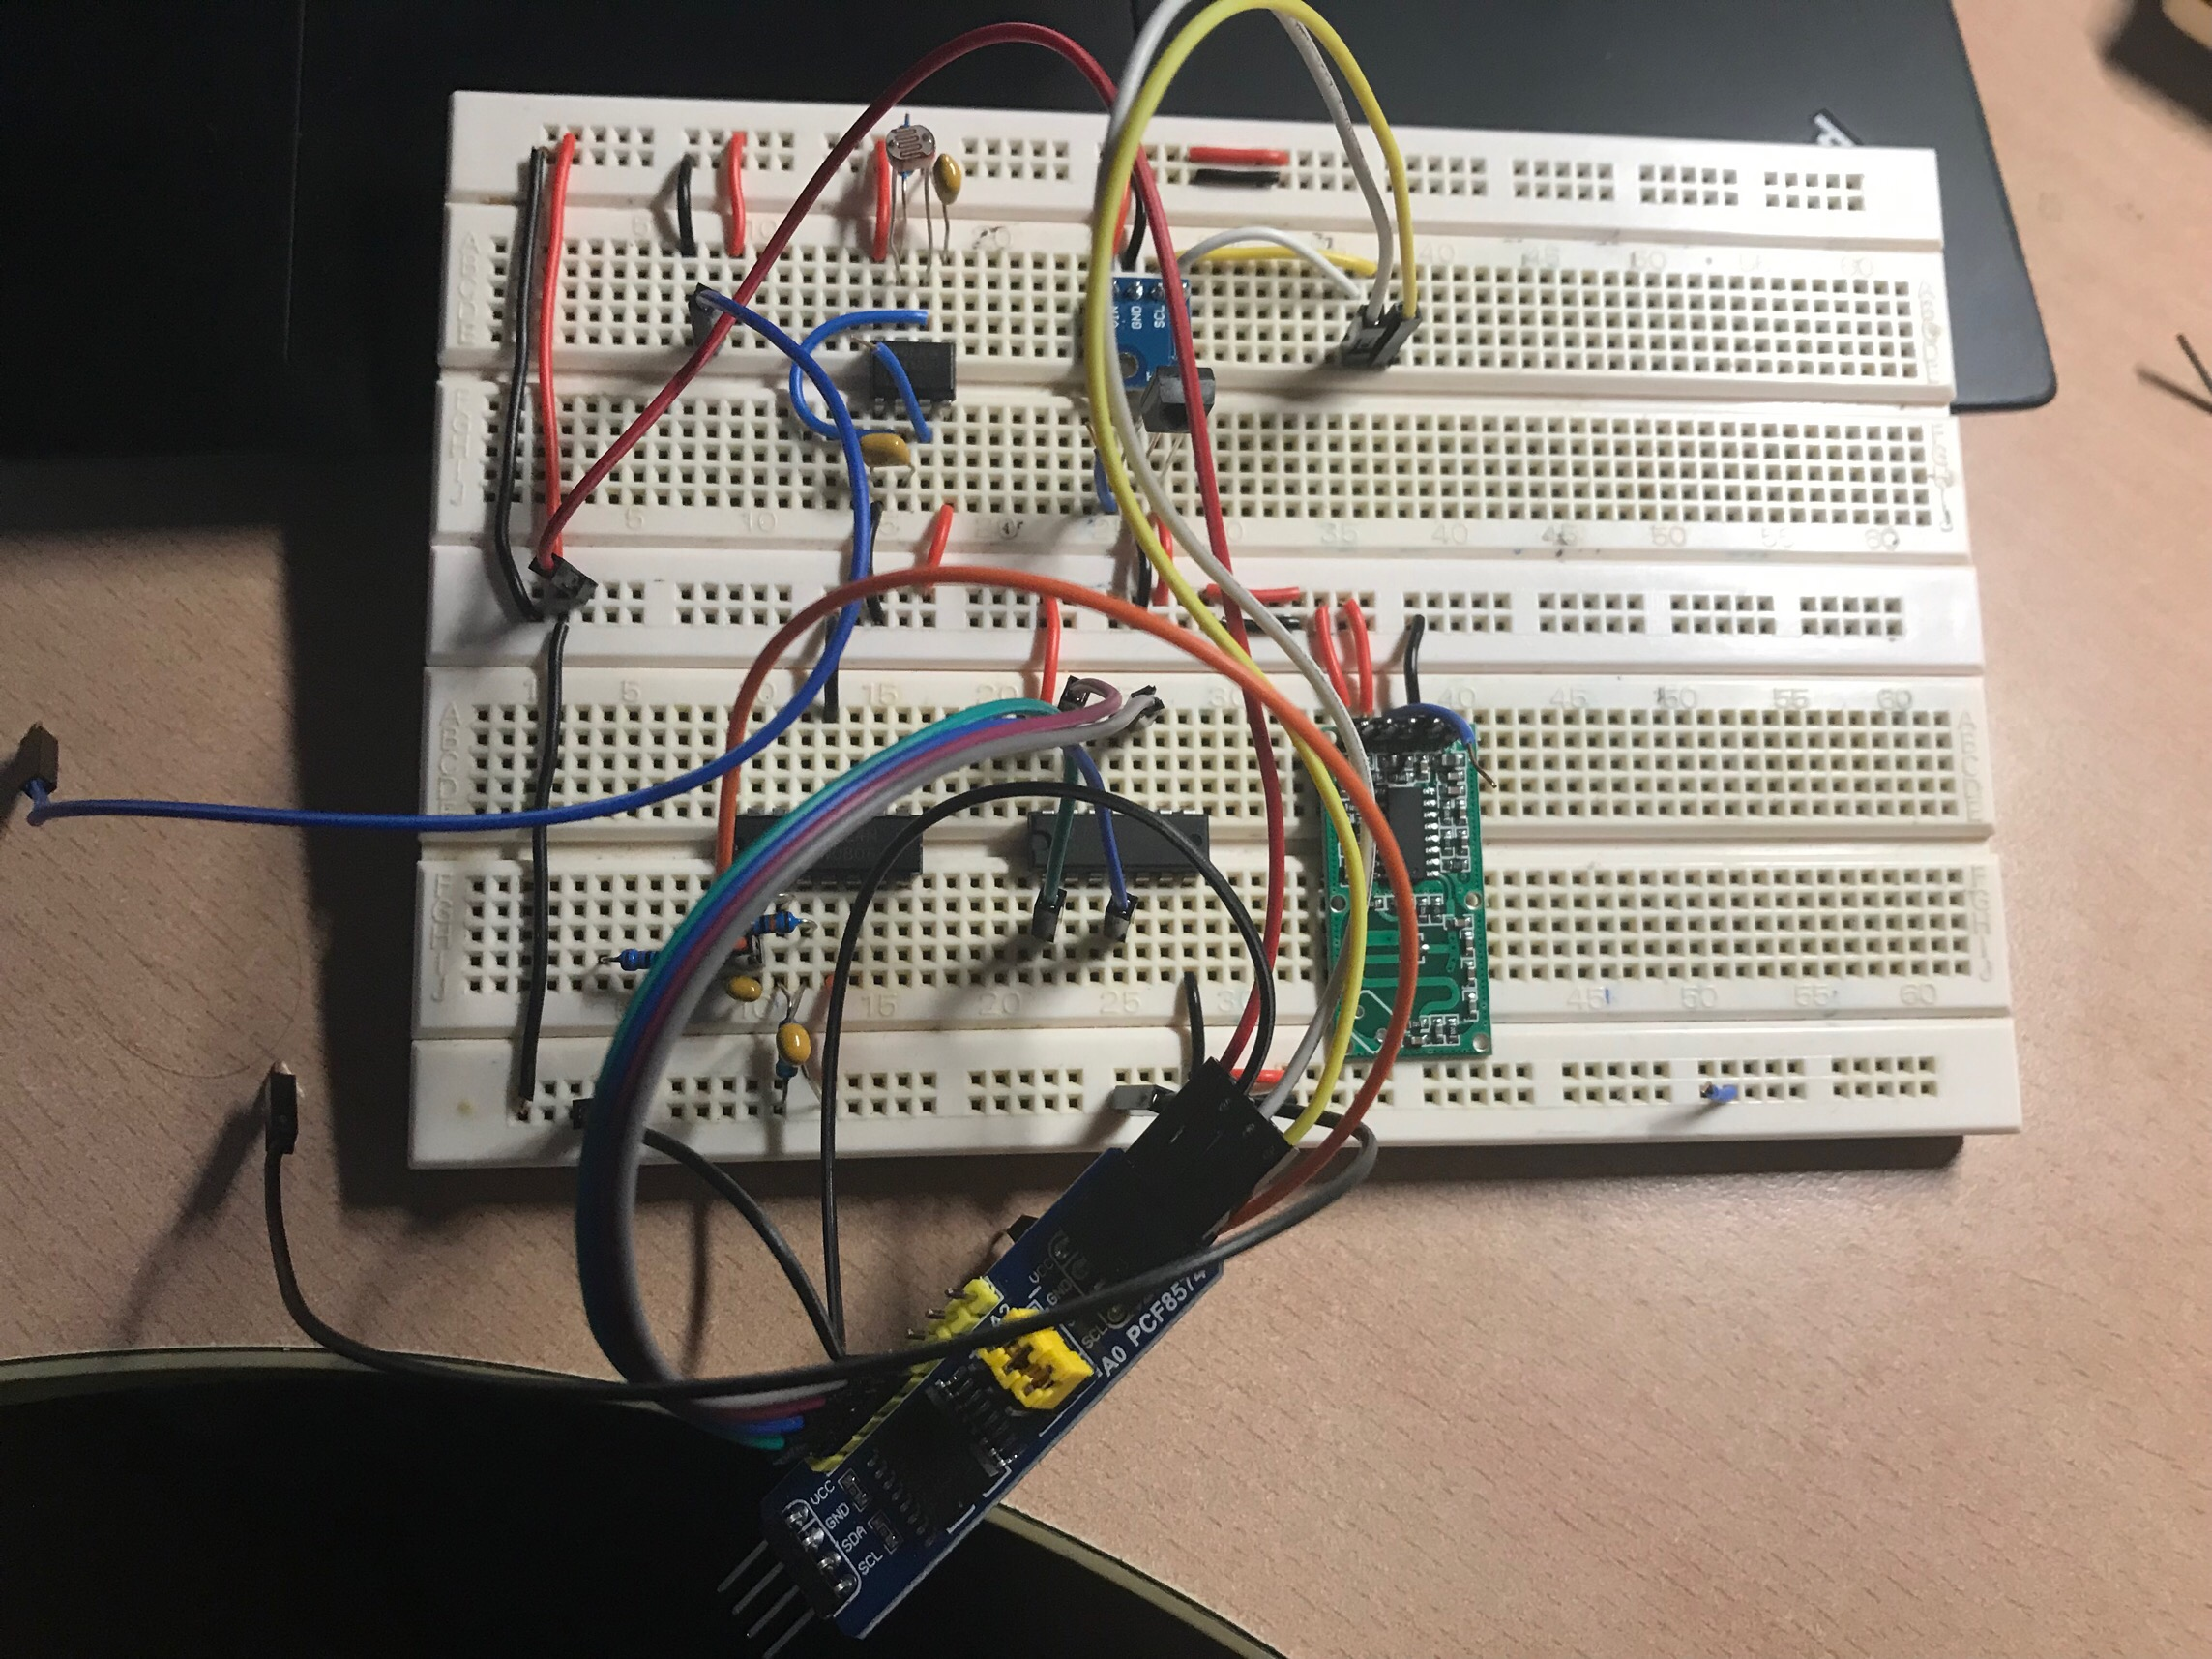
\includegraphics[width = 0.618\textwidth]{all_outside_circuit.jpg}
  \caption{外围电路联调}
\end{figure}

另一路在进行PCB板焊接时,由于按钮插孔的焊盘过小,我们失手将其焊落,难以进行修补。这给了我们一定的教训,PCB印制结束后,并不意味着工序的结束,在实验的任何一个阶段都要小心操作。为了保证进度,达成本周实验结束后将外围硬件部分联调通过,方便周末写软件部分的目的,我们选择换用万能板做电源管理模块,迅速搭接如下电路,并将电源管理模块加入联调。

\begin{figure}[H]
  \centering
  \includegraphics[width = 0.618\textwidth]{V_src.jpg}
  \caption{电源管理模块实物}
\end{figure}

最后在用示波器简单验证各模块输出,再辅助简单的串口打印检测量的程序,我们验证了外围电路联调的基本通过,给周末进行软件部分调试打好了坚实的基础。
\end{diary}


\begin{diary}{2019.07.06上午}{联合检测代码与元件采购}
\par{}在经过周五的电源的准备,为我们的联合调试提供了基础,我们进一步推动了工作的进度,开始想办法在节省动态内存的情况下编写代码,首先我们在检测部分进行联合调试,我们结合了温度湿度气压与灰尘和基于555的光强检测在串口显示数据。

而在上午的调试过程中我们遇到了DHT11模块显示不准的问题,我们在测试的过程中发现了串口显示的温度要明显的高于室温5$^{\circ}C$左右的,并且会在checksum的时候报告checksum error,据查阅是串口数据传输的校验位错误,而我们在仔细研究了dht11.h的库后发现旧版本的dht库函数在检验sum和中将小数部分当做零处理,而我们现在使用的传感器小数部分并不等于0,将其进行如下所示的修改便可:
\begin{figure}[H]
  \centering
  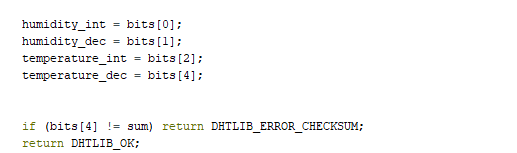
\includegraphics[width = 0.618\textwidth]{code.png}
  \caption{库函数修改}
\end{figure}

在修改后明显测量数据在正常的室温范围内,并且相较于起初的单元模块调试,能够精确的小数点后两位,有较大的精度上的改善,除此之外,我们前往中发市场采购了中型的洞洞板,为检测模块的固定进行了进一步的准备。

\end{diary}


\begin{diary}{2019.07.06下午}{通信部分代码编写与焊接设计}
\par{} 在所有的检测模块都能够正常工作后,我们一路进行代码的完善补充另一路进行焊接的设置,首先是代码层面,开始了将蓝牙部分以及舵机和雷达部分接口的设计,并将蓝牙与SD card部分的库与代码加入我们总的debug代码中,进行了编译以及调试,效果良好,并且,我们为了节省内存,查阅了一些arduino编程的技巧以及变量运用的技巧,尽量减少内存的占用。

而另一路则将面包板的检测部分,设计在洞洞板上进行焊接,由于在周五的焊接中发现洞洞板在接线方面不太方便,因此首先查阅了洞洞板焊接的技巧,其中接线主要分为两种方法,其中一种为连焊走锡式焊法,通过焊锡来使电气连接,另一种方法为背面飞线式,通过导线在洞洞板背面实现电气连接,由于走锡式焊法极易造成错误,难以修改,因此我们决定采用飞线式焊法,并且做了以下简单的设计:

\begin{figure}[H]
  \centering
  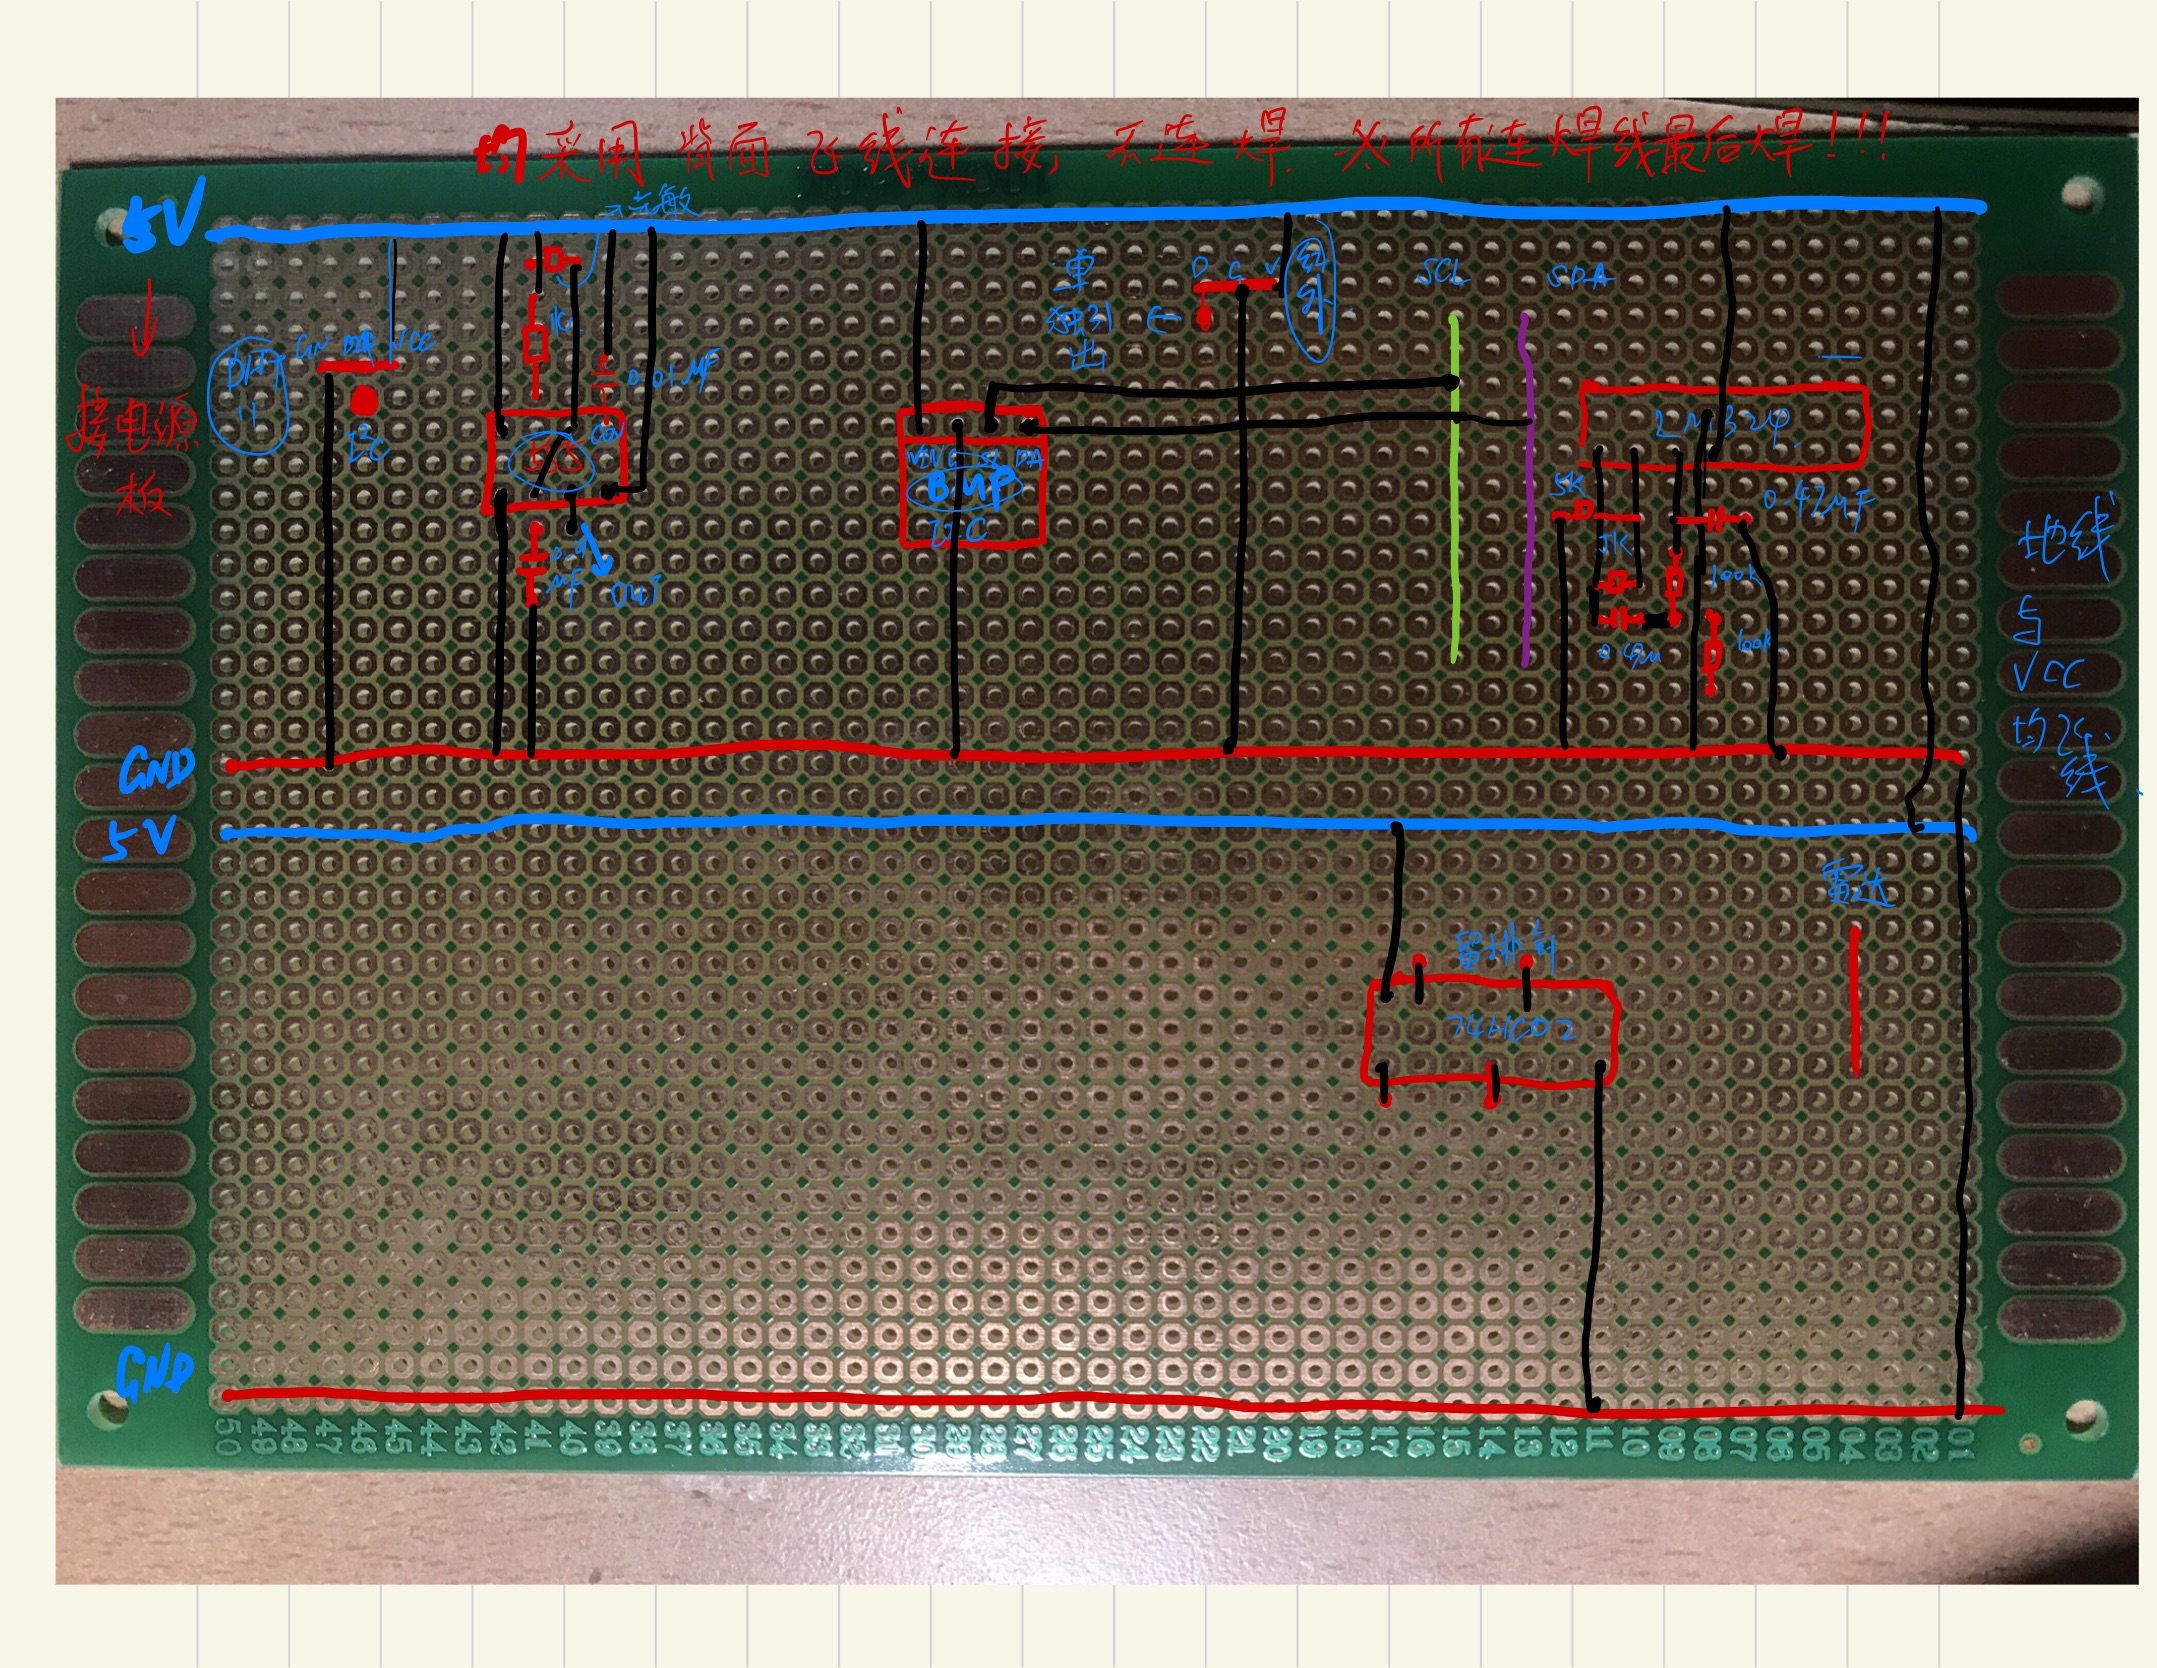
\includegraphics[width = 0.618\textwidth]{han.jpg}
  \caption{焊接简单设计}
\end{figure}
我们此板打算只焊接检测部分,并且电源管理部分单独用一块小板,显示部分另用一块板进行共地处理。

\end{diary}

\begin{diary}{2019.07.07上午}{显示方法设计讨论与代码完善}

在电子设计小学期第六天的上午,我们在其他模块的代码完成后,开始了显示部分的讨论,首先是硬件上对显示的控制,我们列举了需要显示的内容:温度,湿度,气压,灰尘,雷达监测、光强这六项内容,初步设计通过四个独立按键来控制,由于LCD1602仅为16*2的显示,因此每一个测量指标需要占用一行,我们采用翻页设置,分别利用两个按键进行上翻和下翻,另一个按键为滚屏的开始/停止键,滚动屏幕每次滚动一行,另一按键为灵敏度调节,开启此按键后,通过另一电位器调节检测周期,我们设计基准的周期为1s。而另一方面利用红外遥控进行同样的控制,另外单独通过按键来改变显示的顺序,同样通过蓝牙进行串口的数据传输,类似于电脑的串口监视器。这是我们对于显示部分的讨论结果。

在讨论结果设计好后,便开始将显示部分加入我们的主代码,具体使用的函数见于报告附的代码中,基本的实现方法和我们模块调试大同小异,只是在翻页设置我们添加了状态与按键编码的练习,通过逻辑运算来切换状态,至此我们已经完成了整体的所有部分的代码,动态内存也达到了$73\%$,即将到的$75\%$的阈值。只需在周一进行代码的测试。

\end{diary}



\begin{diary}{2019.07.07下午}{混沌电路的设计以及独立按键硬件设计}

在完成了整体代码的设计后,我们便需要在硬件部分进行设计,也即我们设计的独立按键的四个功能:滚屏、上下翻页和灵敏度调节。我们所需要的是在按下时得到其高电平,因此我们可以通过对四个键进行编码,经过IO转I2C接口后直接以I2C形式给到Arduino的SDA和SCL,在内部对其进行地址分配即可,我们通过四个独立按键给出的编码来进行状态的切换,而设计以简单为原则,参照FPGA独立按键的原理,采用上拉电阻和下拉电阻便可简单的解决问题。
\begin{figure}[H]
  \centering
  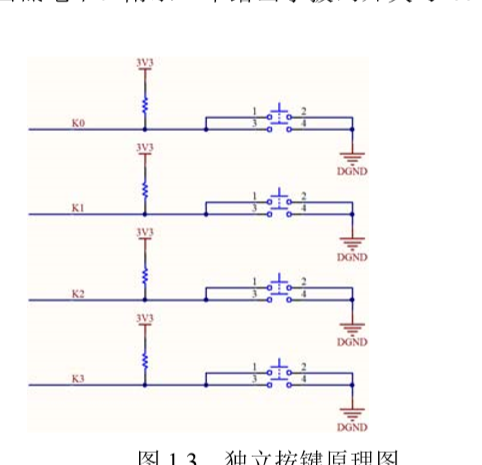
\includegraphics[width = 0.48\textwidth]{dianping.png}
  \caption{独立按键设计}
\end{figure}

这部分设计比较简单,因此还需明天在实验室进行显示、通信、检测三大部分的联合调试,再具体的发现问题。

除此之外,由于雷达需要进行旋转扫描,而针对于室内情况,随机角度的扫描更符合对环境检测的需求,而不是定时的进行旋转,因此舵机旋转角度的设置便可有产生随机数来进行确定,我们初步的思路为产生电压值随机的模拟电压,通过Arduino的模拟接口来读入模拟电压在程序内部进行进一步的随机角度设置。

但设计的关键之处在于随机电压的产生,我们在查找文献后找到了一种混沌电路的发生方法,其原理为使用RC振荡电路但使其震荡点不稳定从而使振荡频率非周期变化,来产生混沌。其原理电路如下:
\begin{figure}[H]
  \centering
  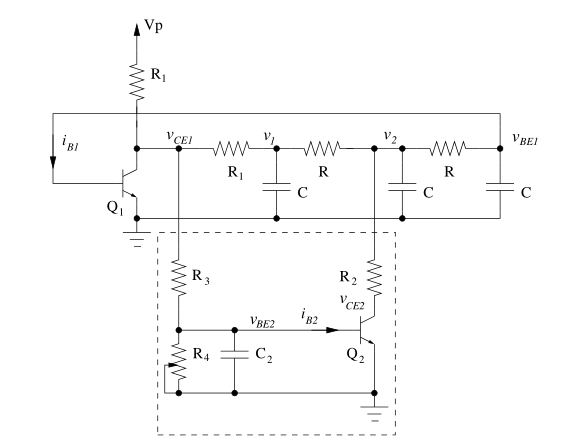
\includegraphics[width = 0.58\textwidth]{hundun.png}
  \caption{混沌电路}
\end{figure}

在修改其参数便于实验室中找到已有元件后,得到稍规律化后的混沌电路,但观察其相图仍为混沌状态,仿真结果如下:
\begin{figure}[H]
  \centering
  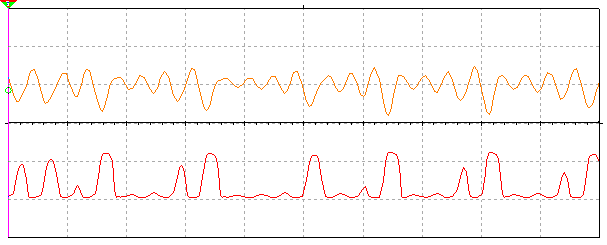
\includegraphics[width = 0.58\textwidth]{hundun1.png}
  \caption{混沌电路仿真}
\end{figure}

我们进一步在面包板上搭建了混沌电路,计划周一上工后利用电位器进行调节到混沌状态,至此我们周末的调试基本结束,总体的代码也已基本完成,若在周一所有模块联调后正常工作,我们便进行焊接与外围电路位置分配的设计。
\end{diary}


\begin{diary}{2019.07.08上午}{联调验证与焊接}

得益于周末的顺利工作,我们上午先在面包板上再次进行验证性的联调,联调通过的模块进行焊接,其他模块继续调试。按照两路并行的模式继续工作。调试时,大部分的检测模块都顺利工作,但是GP2Y灰尘传感器工作不正常。

通过对程序不断注释与控制变量,我们逐次发现了一下几个原因:
\begin{itemize}
  \item arduino与SD卡通信时需要用到SPI总线协议,故除SD卡选通端,其他端口在库中已经写好。而这写好的引脚中的一个与GP2Y传感器使用的LED的IO口发生冲突,导致无法驱动传感器内部的LED进行闪烁,进而检测到的模拟量始终为0,修改了这个错误后,我们直接使用模拟口读入数据在正常范围内。
  \item 滤波后输出过低。使用示波器观察比照低通滤波前后的波形发现我们之前的滤波手段并不正确。为保护红外管,GP2Y1050数据手册建议的是需要采样时,按照给LED一个脉冲,在脉冲末端读取模拟输出,且建议的检测LED闪烁时长不得少于$10ms$,采样点在LED启动后$280ms$之后。而之前的截止频率在过低,导致低通滤波直接将检测信号的很多有效分量滤除,自然无法检测到模拟量,因此我们修改了参数的设置,将截止频率设置在$3kHz$以上。此外,还发现了之前的通带放大倍数为2,在传感器模拟端口输出较大,大于$2.5V$时,2倍的通带放大倍数可能导致输出信号大于$5V$,会在检测浓度较高时超出1023的量程,并且有可能损坏主控板模拟输入口。因此,我们将通带放大倍数修改为1,也即滤波器通带等效为电压跟随器,对应修改其他电阻,保证NP间的直流通路下,对地电阻相同,保证直流对称即可。
\end{itemize}


\end{diary}



\begin{diary}{2019.07.08下午}{遥控测试、混沌电路调试与万能板焊接}
\par{}


下午继续兵分两路的工作,一路进行模块测试,一路进行模块焊接,将测试通过的模块逐个焊接到万能板上。首先是调试的部分,在红外遥控控制的调试中遇到了一些小问题,例如state的变化并非和按下的按键相匹配,经查找后发现是代码中逻辑运算优先级的问题:
\begin{figure}[H]
  \centering
  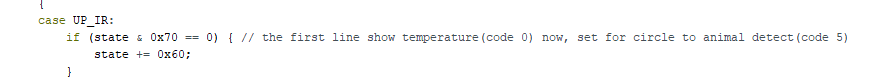
\includegraphics[width = 0.618\textwidth]{code1.png}
  \caption{红外遥控编码}
\end{figure}
如上图所示由于运算优先运算后面的等于号,再运算按位与,和我们的初衷相反,因此我们手动修改运算优先级后解决了问题,并且通过和LCD显示的联调可以通过遥控实现上下翻页和滚屏的开始与停止操作,因此红外模块也可以交去焊接。

在红外调试之后,开始了另一部分模拟电路的调试,也即昨天所设计舵机转动的混沌电路,而我们在调试的过程中始终无法使其产生平衡点不稳定的振荡,总是出现一定的周期化,我们检查了三极管的连接,使用参数的阻值,不断修改电位器,不断重新仿真,始终没有得到混沌的输出。


而焊接部分则是比较消耗时间的部分,由于焊接人数众多,因此不得不有很多的等待时间,不过我们对于模块的焊接短短续续持续了一整天,并且想要通过排针来引出data端,既方便又美观。至此,我们已经焊接完成的模块是DHT11检测部分,PM2.5检测部分,红外遥控部分,基于555的光强检测部分,PM2.5VCVS低通滤波检测,舵机部分,电源管理电路部分,如下图所示:
\begin{figure}[H]
  \centering
  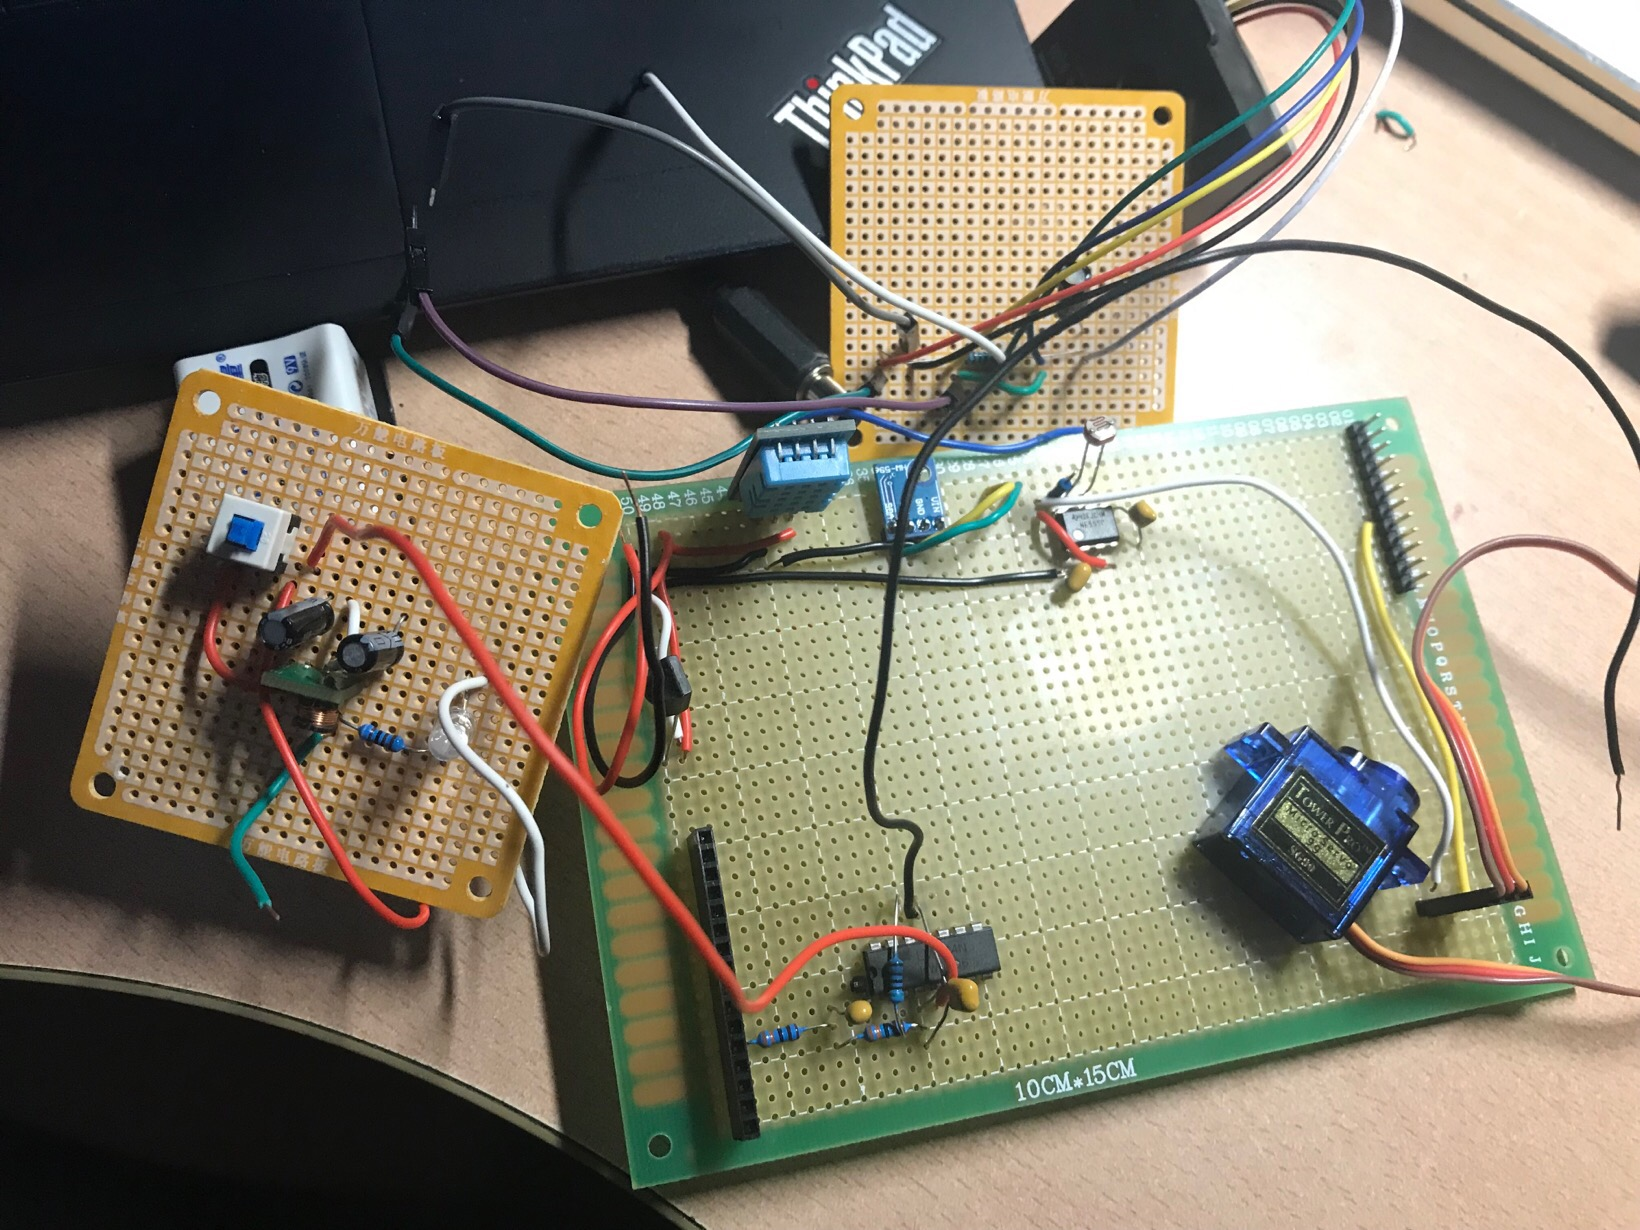
\includegraphics[width = 0.618\textwidth]{hanjie.jpg}
  \caption{焊接成果}
\end{figure}

临近5点,我们还有部分,待收尾的工作有:混沌电路的调试和部分连接点的焊接。我们决定在晚上解决这些问题,保证进度,方便明天的调试。

\end{diary}

\begin{diary}{2019.07.09上午}{焊接与中断源}

在昨晚的焊接之后,我们将模块基本固化到了万能板上面,在早上进行简单的联调后,发现除了带动雷达的舵机不转和灰尘传感器的滤波输出不正常之外,其他模块工作正常,与数字系统联调能正常工作。于是我们开始进行这些问题模块的排查。另一方面,我们注意到我们设计的系统需要的采样频率不高,而使用数字系统本身的延时函数进行轮询的周期的调节,一方面程序复杂,另一方面延时时,单片机仍然工作在正常状态,功耗较大。

在简单讨论后,我们决定设计一个长周期的方波发生器,作为中断输入,而单片机调用下级传感器的做采样的函数,即作为中断服务程序,这样在非采样时,数字系统可以工作在睡眠状态,有效降低功耗,也可以解决LCD在更新时的闪烁问题。从这里,我们进一步为系统增加了一个功能,即自动采样和手动采样,用一个开关切换方波输出和另一个555单稳态电路输出,后者作为即可作为手动采样的触发信号,这样可以帮助使用者标定房间内不同地方的相关参数。
  
\end{diary}

\begin{diary}{2019.07.09下午}{焊接与排错}

上午舵机不工作和滤波器输出异常的错误,经过仔细的排查,发现是这两个元件的地端未接好,用示波器显示为约$5V$,再经过排查,发现是地线那部分出现了虚焊,与电源管理模块共同作用,导致了一定的浮动电压,进而导致运放输出基准变为$5V$,故而滤波后输出总是出现超过测量范围的异常。而舵机两端相当于没有供电,也因此不转。在搞清楚问题后,我们对那一部分重新焊接,排除了错误。

此外,下午的焊接也有很大收获,我们基本完成了焊接,决定晚上进行收尾联调和包装盒的制作。
    
\end{diary}

\begin{diary}{2019.07.10上午}{首次验收和第二次验收}
  
上午一到,进行简单的联调复现,我们进行了首次验收,主要实现的功能有:

\begin{itemize}
  \item 5个物理量的测量,包括温度、湿度、气压、光强和PM2.5颗粒物浓度。
  \item 做一定的有效换算,如把气压转换为标准大气压、光强用为科学计数法、PM2.5浓度到空气质量指数的换算并且显示。
  \item 实现了一定的状态切换与显示,可以让LCD进行滚动显示和手动翻页的切换。
\end{itemize}

在第一次验收通过后,极大的增强了我们的信心,按照预计方案,我们将各数值的采样作为一个采样用的总函数题,用两路切换的,加入滑动变阻器的555多谐振荡电路、555单稳态电路,作为可调时长的自动采样和手动采样功能,进行调试。这样中断触发的形式,还能让arduino进入睡眠模式,让整体系统功耗更低,使用时间更长。完成了增加的功能,并且由此进行了第二次验收。助教也认为认为自动手动采样的功能比较符合我们设计的测量仪器的功能要求,并且建议我们在装箱后,给伸出的用于调节采样市场的滑动变阻器周围进行时长定标,让仪器使用更人性化。

\end{diary}

\begin{diary}{2019.07.10下午}{电路故障排查与存储功能、蓝牙通信、上位机通信验收}

在经过上午的验收后,我们的电池很快没电,在充电后再次上电发现出现了我们长遇到的问题,DHT11的LED在未通电时便亮了,这直接告诉我们出现了共地错误,而我们不加电池模块时,便没有出现这个问题,我们将问题聚焦在电池模块,经过万用表各个共地点排查,发现了电池的地和Arduino的地之间有2.4V左右的电压,而我们经过测量,发现Arduino地线良好,而电池连接线地线也同样是电气短接的,这着实让人困惑,我们这时已经怀疑是电池座的问题,无奈先剪短了已经焊接的和电源管理部分的连接,开始单独排查电源和Arduino,现象非常显然,电池无法通过供电口驱动Arduino,且此时电池已经充满电,在找助教寻求帮助后确认是电池盒地线内部可能发现断接或连接不牢,换了电池盒立刻解决了问题,也让已经验收过的我们对此类问题更加警觉与重视。

在恢复了功能后,我们开始调试SD卡存储功能,通过将数据以csv的格式存储在sd card上,我们以电位器调节到10s的采样周期,读取了约400组数据进行简单的分析,我们本想利用R语言对其进行因子分析(FA),以求通过更少的维度来作为描述室内环境的舒适度指标,但很遗憾在探索性数据分析后发现数据变化范围极小,表现为scattermatrix的极小相关性,很难进行降维,因此我们不得不放弃这个想法。

之后我们进行了第三次验收,这一次我们向助教展示了蓝牙通信功能,可以在手机实时监视串口传送的数据,和之前已经试验过的sd卡存储。之后我们将暂时放弃红外接收功能,调试雷达模块,也即我们测试的第六个物理量,但是雷达模块工作不如我们所愿,其检测过于敏感,不符合我们的预期。

除此之外,我们对电路进行了一些补焊接,引出了一排VCC和一排GND,希望将电路的杜邦线连接尽量规整,并且初步测量规划为其装箱。

\end{diary}
\begin{diary}{2019.07.11上午}{性能指标验收和展示ppt制作}

在电子设计小学期的最后一个工作日上午,我们的设计已经基本验收完成,然而还缺乏对应的精度与性能指标。值得一提的是,在经过昨晚的手工制作后,我们的设计已经装箱完成,为其固定了各个模块在箱中的位置,装箱效果如下图所示:
\begin{figure}[H]
  \centering
  \includegraphics[width = 0.618\textwidth]{zhuangxiang.jpg}
  \caption{装箱效果}
\end{figure}
在前一晚我们在宿舍调试好了舵机与混沌电路,希望将微波雷达模块装载在舵机上能够随机转动进行扫描,而发现雷达模块在检测到移动物体产生上升沿后不会下降,可能是由于雷达对于7米范围内的移动人体过于敏感,但始终无法达到我们的检测效果,因此不得不放弃雷达模块。

我们向助教展示了我们的装箱效果,由于起初焊接设计时并未考虑如何装箱,导致在对键盘模块进行装箱时有些困难。其次,我们计算了PM2.5模块的检测精度,由于我们没有标准pm2.5检测仪,并且直接使用模块来进行示数,也无从进行标定,我们通过转化为浓度值,再转化为标准空气质量对照表,最后根据datasheet来计算其精度与误差,光强检测模块同样无法标定,由于无标准元件作为基准。而BMP采用同样方法计算精度,DHT11则直接给出了精度的范围,这便计算了我们全部模块的性能指标。

在验收过后,也是我们的最后一次验收,这时我们便开始了ppt的制作。
\end{diary}

\begin{diary}{2019.07.11下午}{展示ppt制作与元件盒归还}

在下午时,我们回来后首先将元件盒归还,将元件整理到新的泡沫板上,紧接着在小组两人都归还元件盒后,我们同时开始了ppt的制作,很快两人就将ppt的内容以及我们在所有的调试中遇到的问题总结清楚,并完成了交流答辩ppt的制作,进一步分工明天如何展示。
\begin{figure}[H]
  \centering
  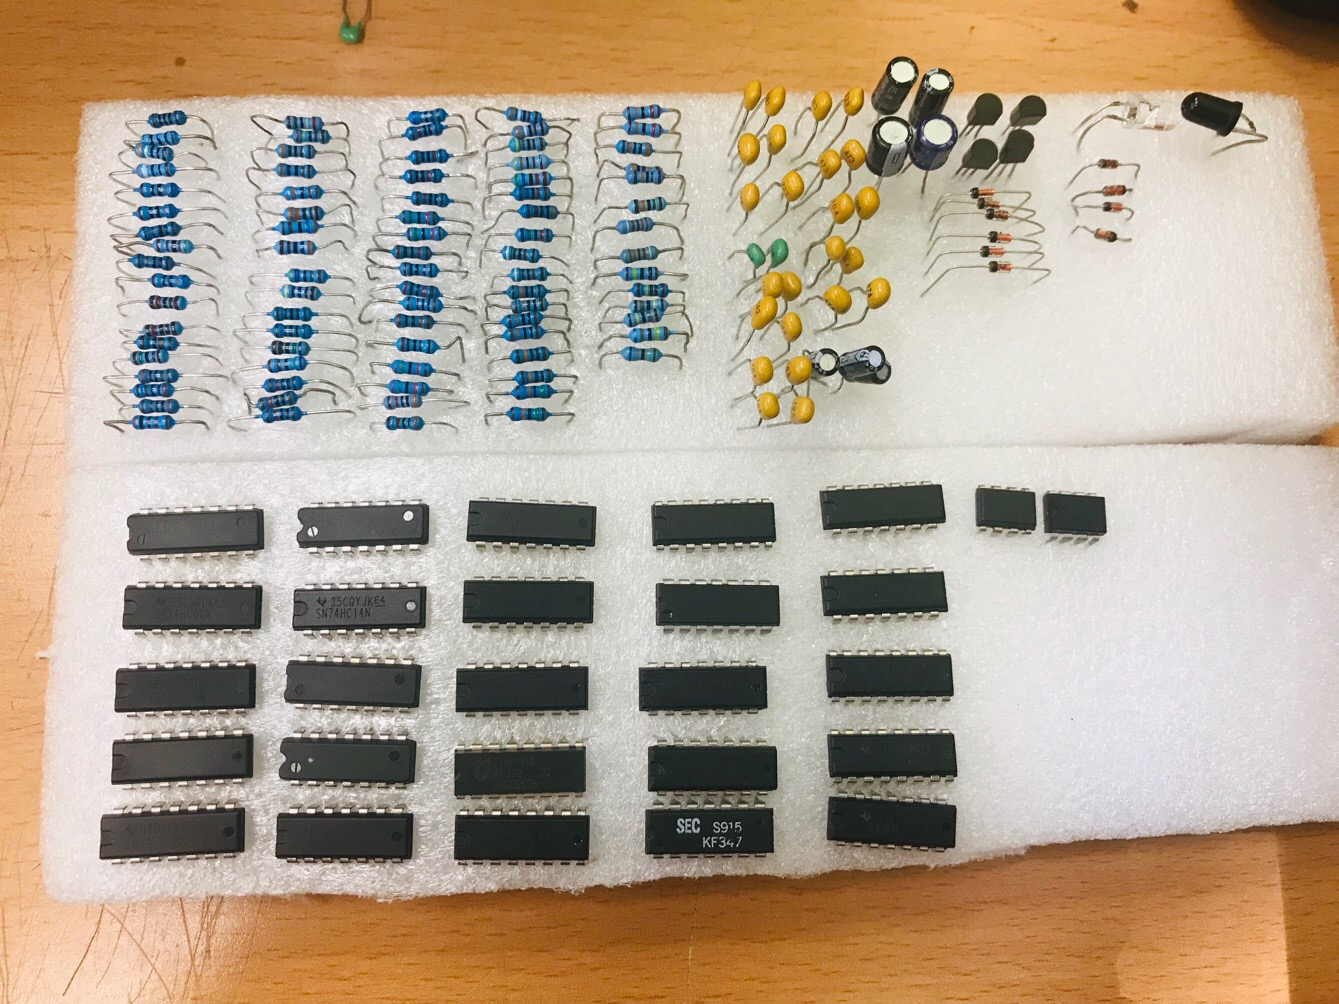
\includegraphics[width = 0.58\textwidth]{yuanjian.jpg}
  \caption{元件归还}
\end{figure}
在交流答辩ppt的制作中,我们重新绘制了电路框图,而在预习报告绘图的基础上进行添加,相比于预习,实际上在控制方面添加了不少内容,也增添了更多的模拟电路部分。

下午的工作较早结束,我们也便观摩了其他组同学的产品,并且私下里了解了其他同学的设计思路和调试遇到的问题,这让我们组受益匪浅,总而言之,我们的验收也已经完成,尽管有许多的不足以及改进空间,但总归顺利完成了我们预习时初步预想的效果,电子小学期最后一个工作日就这样结束,也祝我们明天的交流答辩顺利!


\end{diary}
\end{document}
